\documentclass[12pt,a4paper]{article}

% Русский язык
\usepackage[T2A]{fontenc}
\usepackage[utf8]{inputenc}
\usepackage[russian]{babel}

% Математика и графика
\usepackage{amsmath,amssymb}
\usepackage{graphicx}
\usepackage{float}

% Таблицы
\usepackage{tabularx}
\usepackage{booktabs}
\usepackage{array}
\usepackage{caption}
\captionsetup[table]{justification=raggedleft,singlelinecheck=false}
\setlength{\tabcolsep}{4pt}

% Ссылки и оглавление
\usepackage[hidelinks]{hyperref}
\usepackage{tocloft}


% Листинги кода
\usepackage{listings}
\usepackage{fancyvrb}
\lstset{
    basicstyle=\ttfamily\small,
    breaklines=true,
    frame=single,
    literate=
      {—}{{--}}1
      {←}{{$\leftarrow$}}1
      {→}{{$\rightarrow$}}1
}

% Геометрия и отступы
\usepackage{geometry}
\geometry{left=2.5cm,right=2.5cm,top=2cm,bottom=2cm}
\setlength{\parindent}{1.25cm}
\setlength{\parskip}{0pt}

% Формат заголовков
\usepackage{titlesec}
\titleformat{\section}{\large\bfseries}{\thesection}{1em}{}
\titleformat{\subsection}{\normalsize\bfseries}{\thesubsection}{1em}{}

\begin{document}

% Титульный лист
\begin{titlepage}
    \centering
    {\large \textbf{САНКТ-ПЕТЕРБУРГСКИЙ ГОСУДАРСТВЕННЫЙ УНИВЕРСИТЕТ}} \\[0.5cm]
    {\large Факультет прикладной математики--процессов управления} \\[0.5cm]
    {\large Программа бакалавриата} \\[0.2cm]
    {\large \textbf{«Большие данные и распределенная цифровая платформа»}} \\[4.5cm]

    {\Large \textbf{ОТЧЕТ}} \\[0.3cm]
    {\large По проектной работе} \\[0.2cm]
    {\large По дисциплине «Алгоритмы и структуры данных»} \\[0.2cm]
    {\large На тему «Распознавание рукописаного текста и анализ эмоциональной окраски»} \\[4cm]

    \begin{flushright}
        Студенты гр. 24Б15-пу \\ [0.5cm]
        Телицин А.Д. \\
        Шаймиев К.А. \\[1cm]
        Преподаватели \\ [0.5cm]
        Дик А.Г. \\
        Щеголева Н.Л. \\[1cm]
    \end{flushright}

    \vfill
    \centering
    Санкт-Петербург \\
    2026 г.
\end{titlepage}

\tableofcontents
\newpage

\section{Актуальность}
\label{sec:relevance}

В эпоху цифровизации автоматическая обработка рукописных документов, таких как архивы, письма и анкеты, становится все более востребованной. Технологии распознавания рукописного текста (HTR) позволяют переводить их в цифровой формат, открывая возможности для анализа и поиска.

Однако для глубокого понимания содержания простого распознавания недостаточно. Анализ эмоциональной окраски (тональности) извлекает из текста субъективную информацию — настроение и отношение автора, что критически важно для социологии, психологии и исторических исследований.

Совмещение распознавания рукописного текста с анализом его тональности является сложной и актуальной задачей. Ее решение позволяет не только оцифровывать аналоговые источники, но и автоматически извлекать из них эмоциональный контекст, что значительно обогащает данные для исследований. Данный проект направлен на создание инструмента, решающего обе эти задачи, что и определяет его актуальность.

\section{Цель работы}
\label{sec:goal}

Целью работы является разработка программного инструмента для автоматического
распознавания рукописаного текста и последующего анализа тональности распознанного
содержания.

\subsection{Задачи}
Для достижения данной цели были поставлены следующие задачи:

\begin{enumerate}
    \item Проанализировать существующие подходы к распознаванию рукописного текста и анализу тональности.
    \item Подобрать и подготовить датасет для обучения и тестирования модели.
    \item Определить метрики качества и критерии успешности решения.
    \item Разработать и реализовать модель распознавания рукописного текста.
\end{enumerate}

\section{Теоретическая часть}
\label{sec:theory}

В этом разделе приведены ключевые термины и методы, используемые в проекте
распознавания рукописного текста и анализа эмоциональной окраски. Далее
они будут использоваться для описания архитектуры модели, процесса
обучения и оценки качества.

\subsection{Распознавание текста и предобработка}

\begin{description}
    \item[Оптическое распознавание символов (OCR, Optical Character Recognition)]
    Автоматическое преобразование изображения с текстом в цифровую строку.
    \textit{В проекте:} используется для распознавания рукописных записей на русском и английском языках.

    \item[Распознавание рукописного текста (HTR, Handwritten Text Recognition)]
    Частный случай OCR для рукописного ввода, более сложный из-за вариативности почерка.
    \textit{В проекте:} основная задача модели.

    \item[Предобработка изображения (image preprocessing)]
    Набор операций перед подачей в модель: снижение шума, выравнивание контраста, нормализация масштаба.
    \textit{В проекте:} оттенки серого, обрезка по содержимому, изменение размера, нормализация, бинаризация и удаление шума.

    \item[Изображение в оттенках серого (grayscale image)]
    Формат, где пиксель хранит только яркость.
    \textit{В проекте:} используется для упрощения обработки и снижения размера данных, так как цвет текста несущественен.

    \item[Нормализация изображения (image normalization)]
    Приведение значений пикселей к единому диапазону.
    \textit{В проекте:} стабилизирует входные данные нейросети.

    \item[Обрезка по содержимому (content crop)]
    Удаление пустых полей вокруг текста.
    \textit{В проекте:} повышает долю полезной информации во входе модели.

    \item[Бинаризация (binarization)]
    Преобразование изображения в черно-белый вид по порогу.
    \textit{В проекте:} используется как дополнительный режим, может как улучшать, так и ухудшать качество при неверном пороге.

    \item[Связная компонента (connected component)]
    Группа соседних пикселей в бинарном изображении.
    \textit{В проекте:} используется для выделения отдельных символов при сегментации.

    \item[Сегментация (segmentation)]
    Разбиение изображения на строки/слова/фрагменты \cite{segmentation2009}.
    \textit{В проекте:} применяется для распознавания частей строки с последующей сборкой результата.

    \item[Профиль чернил (ink profile)]
    Распределение темных пикселей по строкам или столбцам.
    \textit{В проекте:} используется для поиска границ строк и слов без отдельной модели сегментации.
\end{description}

\subsection{Нейросетевая архитектура OCR}

\begin{description}
    \item[Сверточная нейронная сеть (CNN, Convolutional Neural Network)] Является модификацией обычной полносвязной нейронной сети, которая использует
    сверточные слои для извлечения признаков из изображений. Сверточные слои применяют
    фильтры, которые выделяют локальные шаблоны текста, такие как края, углы и текстурные элементы. Это позволяет эффективно распознавать сложные структуры, характерные для рукописного текста.
    \textit{В проекте:} формирует признаки рукописных символов.

    \item[Сверточный слой (convolutional layer)]
    Применяет фильтры к изображению/картам признаков. Является основой CNN.
    \textit{В проекте:} выделяет локальные элементы букв.

    \item[Пулинг (pooling)]
    Уменьшает размер карты признаков с сохранением важной информации.
    \textit{В проекте:} снижает размерность и повышает устойчивость к сдвигам.

    \item[Рекуррентная нейронная сеть (RNN, Recurrent Neural Network)]
    Обрабатывает последовательности с учетом контекста \cite{mdrnn2008}.
    \textit{В проекте:} последовательность - признаки из CNN, контекст - соседние символы.

    \item[Долгая краткосрочная память (LSTM, Long Short-Term Memory)]
    Тип RNN, лучше сохраняющий долгий контекст.
    \textit{В проекте:} помогает различать похожие символы по соседним.

    \item[Двунаправленная LSTM (BiLSTM, Bidirectional LSTM)]
    Анализирует последовательность слева направо и справа налево.
    \textit{В проекте:} учитывает контекст с обеих сторон.

    \item[Сверточно-рекуррентная сеть (CRNN, Convolutional Recurrent Neural Network)]
    Комбинация CNN и RNN для распознавания текста с изображения \cite{survey2023}.
    \textit{В проекте:} основная архитектура для распознавания рукописного текста.

    \item[Тензор (tensor)]
    Многомерный числовой массив.
    \textit{В проекте:} используется для представления изображений и признаков в нейросети.

    \item[CTC-функция потерь (CTC-loss, Connectionist Temporal Classification loss)] \cite{ctc2006}
    Позволяет обучать модель по парам ``изображение--строка'' без посимвольной разметки.
    \textit{В проекте:} ключевой механизм обучения CRNN.

    \item[Декодирование CTC (CTC decoding)]
    Преобразует последовательность вероятностей в текст (с удалением повторов и пустых символов).
    \textit{В проекте:} финальный этап OCR-предсказания.

    \item[Инференс (inference)]
    Процесс использования обученной модели для предсказания на новых данных.
    \textit{В проекте:} применяется для получения результатов распознавания.
\end{description}

\subsection{Датасеты и оценка качества}

\begin{description}
    \item[IAM Handwriting Database]\cite{marti2002iam}
    Набор рукописного английского текста с аннотациями.
    \textit{В проекте:} используется для английского OCR-пайплайна.

    \item[HKR/HTR dataset]\cite{hkr2024}
    Набор рукописного русского текста (изображения + JSON-аннотации).
    \textit{В проекте:} основной датасет для русского OCR.

    \item[Обучающая выборка (training set)]
    Данные для обновления параметров модели.

    \item[Валидационная выборка (validation set)]
    Данные для контроля качества без обновления весов.

    \item[Checkpoint]
    Файл сохраненного состояния модели.
    \textit{В проекте:} позволяет запускать инференс без повторного обучения.

    \item[CER (Character Error Rate)]
    Доля ошибок на уровне символов.

    \item[WER (Word Error Rate)]
    Доля ошибок на уровне слов.

    \item[Расстояние Левенштейна (Levenshtein distance)]
    Минимальное число вставок, удалений и замен для преобразования одной строки в другую.
    \textit{В проекте:} используется при вычислении CER и WER.
\end{description}

\subsection{Постобработка и анализ эмоций}

\begin{description}
    \item[Постобработка текста (text postprocessing)]
    Очистка и нормализация OCR-результата перед дальнейшим анализом.

    \item[Токенизация (tokenization)]
    Разбиение текста на токены (обычно слова).

    \item[Лемматизация (lemmatization)]
    Приведение слов к начальной форме.

    \item[Морфологический анализ на основе pymorphy3]
    Морфологический анализатор русского языка.
    \textit{В проекте:} применяется для лемматизации.

    \item[Коррекция ошибок OCR (OCR error correction)]
    Исправление слов, распознанных с ошибками.

    \item[Триграммное сходство (trigram similarity)]
    Сравнение слов по совпадению трехсимвольных подстрок.
    \textit{В проекте:} используется при подборе корректировок.

    \item[Лексиконный анализ эмоций (lexicon-based emotion analysis)]
    Определение эмоций по словарю с заранее размеченными словами \cite{anew1999,norms2013}.

    \item[RusEmoLex]
    Русскоязычный словарь с эмоциональными метками.
    \textit{В проекте:} источник эмоциональных меток для слов.
\end{description}


\section{Используемые методы и алгоритмы, их пошаговое описание}

\subsection{Общая архитектура программы}
Программа состоит из нескольких основных компонентов:

\begin{itemize}
    \item \textbf{Загрузка датасета:} чтение изображений и аннотаций из выбранного датасета.
    \item \textbf{Предобработка изображения:} преобразование в оттенки серого, повышение контрастности, обрезка по содержимому, изменение размера, нормализация, бинаризация и удаление шума. Приведение к матричному виду для подачи в модель.
    \item \textbf{Обучение CRNN-модели:} сверточно-рекуррентная нейросеть для распознавания текста.
    \item \textbf{Применение обученной модели к изображениям:} преобразование выходов модели в текстовую строку.
    \item \textbf{Постобработка текста (для русского):} токенизация, коррекция OCR-ошибок и лемматизация.
    \item \textbf{Анализ эмоций:} поиск слов в RusEmoLex и вычисление распределения эмоций.
\end{itemize}

\subsubsection{Загрузка датасета}

В качестве основного источника данных для русского языка используется набор данных HKR/HTR,
который содержит изображения рукописного текста и соответствующие JSON-аннотации.
Для английского языка используется база данных рукописного текста IAM (IAM Handwriting Database) \cite{marti2002iam}.

Загрузка данных для русского и английского вариантов не имеет принципиальных отличий,
так как оба набора данных предоставляют изображения и текстовые аннотации. Основные шаги:

\begin{enumerate}
    \item Чтение списка файлов изображений и соответствующих аннотаций.
    \item Сопоставление каждого изображения с его текстовой строкой.
    \item Разделение данных на обучающую, валидационную и тестовую выборки.
\end{enumerate}

\subsubsection{Предобработка изображений}

После загрузки изображения проходят через несколько этапов предобработки:

\begin{enumerate}
    \item \textbf{Преобразование в оттенки серого:} удаление цветовой информации для упрощения анализа.
    \item \textbf{Повышение контрастности:} позволяет повысить различимость штрихов на фоне и удалить артефакты.
    \item \textbf{Обрезка по содержимому:} удаление пустых полей вокруг текста для фокусировки на полезной информации.
    \item \textbf{Изменение размера:} приведение к фиксированной высоте (например, 64 пикселя) с сохранением пропорций.
    \item \textbf{Нормализация:} масштабирование значений пикселей в диапазон [0, 1].
    \item \textbf{Бинаризация (опционально):} преобразование в черно-белый вид по порогу для удаления шума.
    \item \textbf{Приведение к матричному виду:} преобразование изображения в формат, удобный для подачи в нейросеть.
\end{enumerate}

\subsubsection{Обучение CRNN-модели}

В работе используется сверточно-рекуррентная нейросеть (CRNN) из библиотеки PyTorch. Обучение модели происходит на обучающей выборке, а качество контролируется на валидационной выборке.

CRNN-модель состоит из нескольких сверточных слоев для извлечения признаков и рекуррентных слоев для обработки последовательности признаков. Обучение происходит следующим образом:
\begin{enumerate}
    \item Инициализация модели и оптимизатора.
    \item Проход по обучающей выборке в пакетах (батчах) заданного размера.
    \item Для каждого изображения: предобработка и подача в модель.
    \item Получение выходов модели в виде последовательности вероятностей символов.
    \item Вычисление CTC-функции потерь между предсказанием и истинной строкой.
    \item Обратное распространение ошибки и обновление весов модели.
    \item Периодическая оценка на валидационной выборке для контроля качества.
\end{enumerate}

На выходе обучения сохраняется файл, который содержит веса модели (checkpoint), что позволяет
использовать ее для инференса без повторного обучения.

\subsubsection{Применение обученной модели к изображениям}

После обучения модель может быть применена к новым изображениям для получения
текстовой строки. Процесс инференса включает следующие шаги:

\begin{enumerate}
    \item Загрузка сохраненного checkpoint модели.
    \item Предобработка входного изображения аналогично тому, что использовалось при обучении.
    \item Подача изображения в модель и получение последовательности вероятностей символов.
    \item Декодирование CTC для преобразования вероятностей в текстовую строку.
    \item Если применялась сегментация, объединение результатов фрагментов в одну строку.
\end{enumerate}

\subsubsection{Постобработка текста и анализ эмоций}

Для русского текста после получения строки из OCR применяется постобработка:
\begin{enumerate}
    \item \textbf{Токенизация:} разбиение строки на отдельные слова.
    \item \textbf{Коррекция OCR-ошибок:} для каждого слова, не найденного в словаре, поиск наиболее похожего по триграммному сходству и замена на него.
    \item \textbf{Лемматизация:} приведение слов к начальной форме с помощью pymorphy3.
    \item \textbf{Анализ эмоций:} для каждого лемматизированного слова поиск в RusEmoLex и подсчет распределения эмоций по тексту.
\end{enumerate}

После всех этапов программа выводит несколько вариантов распознавания
(с разными режимами предобработки), исправленный текст (для русского)
и информацию о доминирующей эмоции и распределении эмоций в тексте.

\subsection{Используемые алгоритмы}

Вышеперечисленные этапы реализованы с помощью следующих алгоритмов и методов:
\begin{itemize}
    \item \textbf{CRNN (сверточная-рекуррентная нейросеть):} сочетание сверточных и рекуррентных слоев для эффективного распознавания текста с изображений.
    \item \textbf{CTC-алгоритм:} позволяет обучать модель без посимвольной разметки, что критично для рукописного текста.
    \item \textbf{Триграммное сходство:} используется для коррекции OCR-ошибок путем сравнения с лексиконом.
    \item \textbf{Лемматизация:} позволяет привести слова к начальной форме для более точного анализа эмоций.
    \item \textbf{Подсчет распределения эмоций:} суммирование эмоциональных меток из RusEmoLex для определения доминирующей эмоции.
\end{itemize}

Ниже приведено более подробное описание алгоритмов, используемых на каждом этапе.

\subsubsection{CRNN (сверточная-рекуррентная нейросеть)}
CRNN объединяет преимущества сверточных нейросетей (CNN) для извлечения признаков
из изображений и рекуррентных нейросетей (RNN) для обработки последовательностей.
Сверточная нейронная сеть является усовершенствованной версией обычной полносвязной
нейронной сети. Она использует сверточные слои для извлечения локальных признаков из
изображения, что позволяет эффективно распознавать сложные паттерны, такие как
рукописные символы.

Рекуррентная нейронная сеть, в свою очередь, обрабатывает последовательность признаков,
учитывая контекст и взаимосвязи между символами. Это особенно важно для рукописного текста,
где форма символов может сильно варьироваться в зависимости от соседних символов.
В нашем случае архитектура включает:

\begin{itemize}
    \item Несколько сверточных слоев для извлечения признаков. Каждый слой применяет набор
    фильтров к входному изображению или карте признаков, выделяя сложные геометрические шаблоны,
    характерные для рукописного текста.
    \item Пулинг-слои для снижения размерности.
    \item Двунаправленные LSTM-слои для обработки последовательности признаков.
    \item Выходной слой с активацией softmax для получения вероятностей символов.
\end{itemize}

\subsubsection{CTC-алгоритм}
CTC (Connectionist Temporal Classification) — это алгоритм \cite{ctc2006}, который позволяет обучать модели
распознавания текста без необходимости в посимвольной разметке. Он работает следующим образом:
\begin{itemize}
    \item Модель генерирует последовательность вероятностей для каждого символа (включая специальный символ "пусто") на каждом временном шаге.
    Вероятности получаеются на выходе сверточно-рекуррентной нейросети после обработки входного изображения.
    \item CTC-функция потерь вычисляет вероятность правильного распознавания строки, суммируя по всем возможным выравниваниям между входной последовательностью и целевой строкой.
    \item Во время инференса декодирование CTC удаляет повторяющиеся символы и пустые символы, чтобы получить итоговую строку.
\end{itemize}

Преимущество CTC заключается в том, что он позволяет обучать модель на данных, где нет точного выравнивания между входом и выходом, что идеально подходит для рукописного текста.

\subsubsection{Триграммное сходство}

Данный алгоритм используется для коррекции ошибок OCR. Он работает следующим образом:
\begin{itemize}
    \item Для каждого слова, распознанного OCR, которое не найдено в словаре,
    генерируется множество триграмм (последовательностей из трех символов).
    \item Для каждого слова в словаре также генерируются триграммы.
    \item Вычисляется сходство между распознанным словом и каждым словом в 
    словаре на основе количества совпадающих триграмм.
    \item Слово из словаря с наибольшим сходством выбирается в качестве корректировки для распознанного слова.
\end{itemize}

\subsubsection{Лемматизация}

Лемматизация — это процесс приведения слова к его начальной форме (лемме). В нашем проекте для русского языка
используется библиотека pymorphy3, которая предоставляет мощные инструменты для морфологического анализа.
Процесс лемматизации включает следующие шаги:
\begin{itemize}
    \item Для каждого слова, полученного после коррекции OCR-ошибок, вызывается функция лемматизации из pymorphy3.
    \item Библиотека анализирует слово и возвращает его лемму, которая используется для дальнейшего анализа эмоций.
\end{itemize}

\subsubsection{Подсчет распределения эмоций}

Для анализа эмоциональной окраски текста используется лексикон RusEmoLex, который
содержит слова и их эмоциональные метки. Процесс подсчета распределения эмоций
включает следующие шаги:
\begin{itemize}
    \item Для каждого лемматизированного слова выполняется поиск в RusEmoLex.
    \item Если слово найдено, его эмоциональные метки добавляются к общему счетчику для каждой эмоции.
    \item После обработки всех слов вычисляется распределение эмоций, и определяется доминирующая эмоция.
\end{itemize}

\section{Блок-схемы и диаграмма компонентов}

\subsection{Диаграмма компонентов}

\begin{figure}[H]
    \centering
    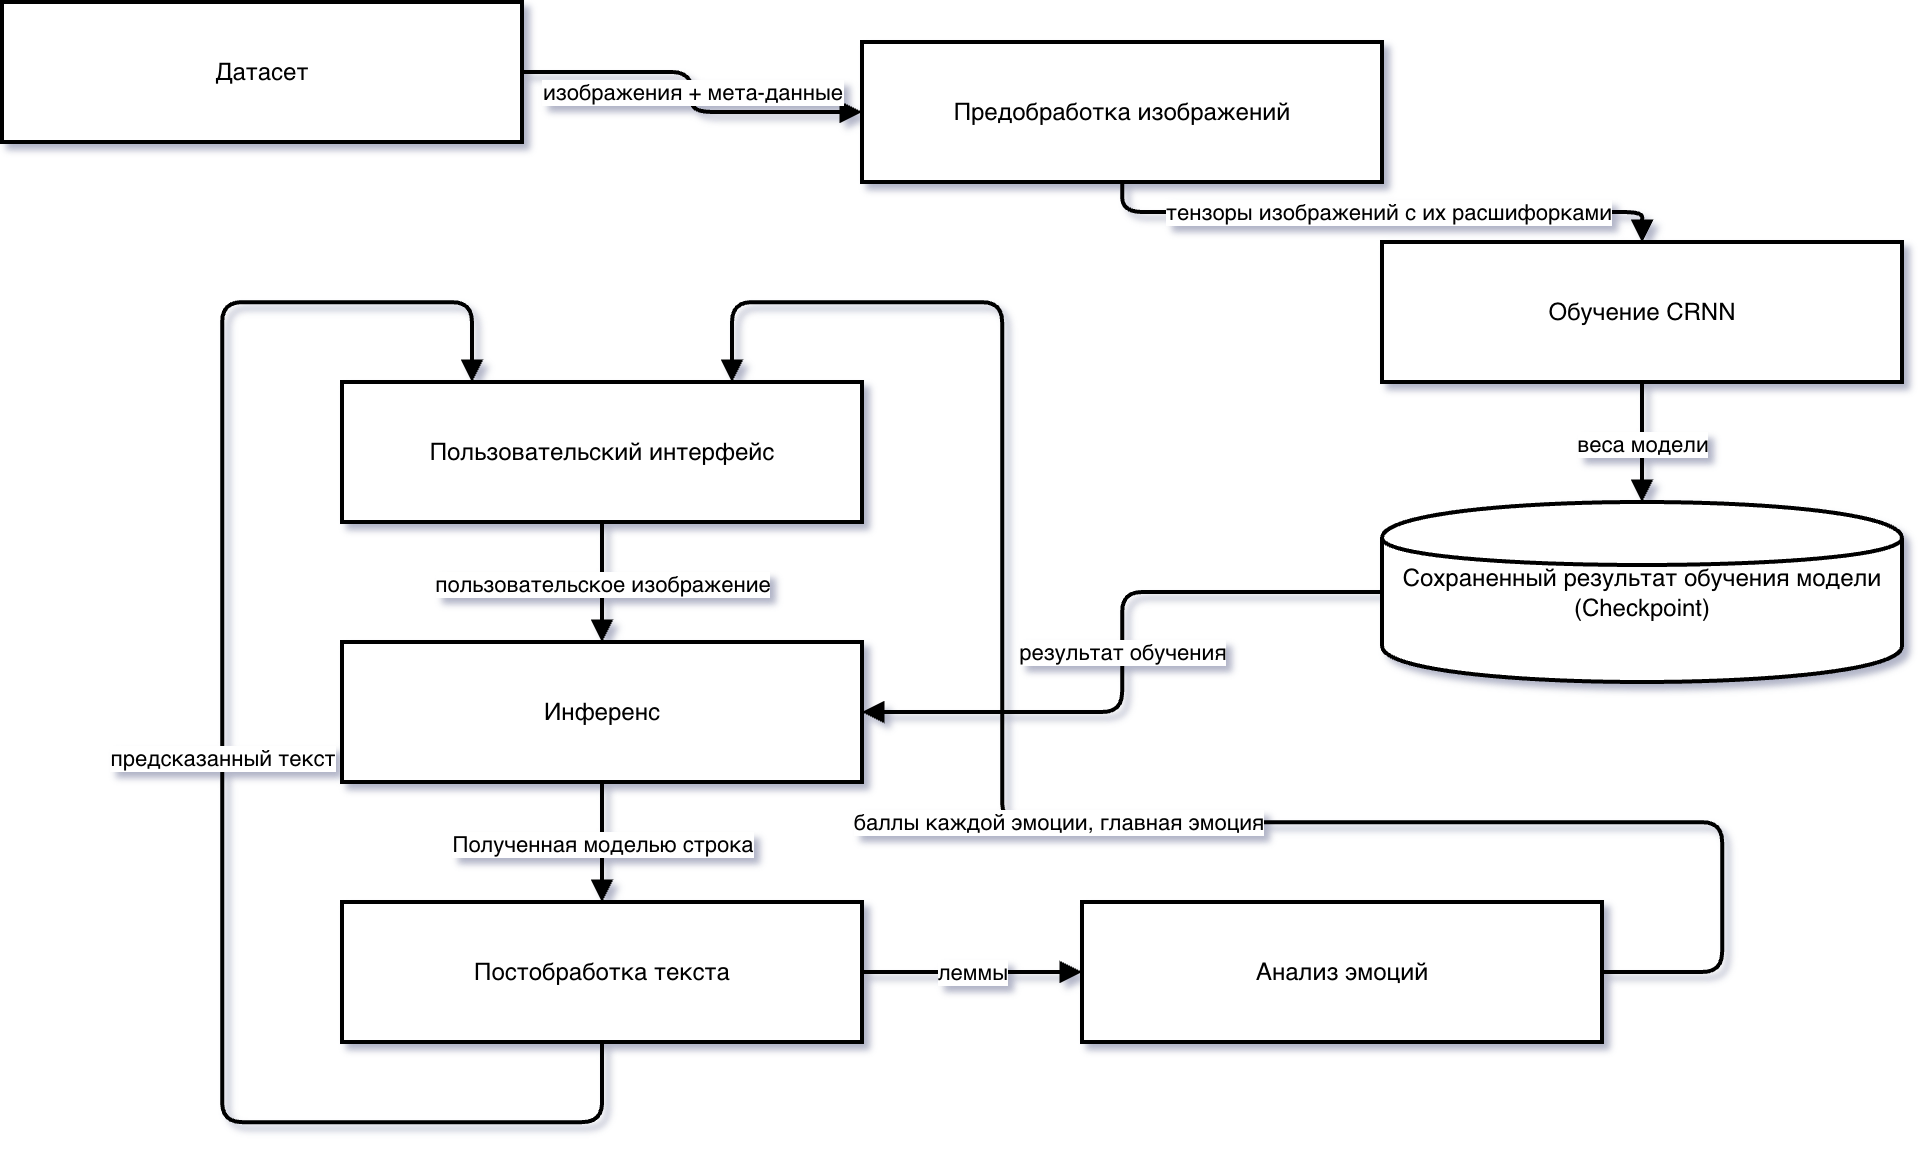
\includegraphics[width=\linewidth]{images/Компоненты.drawio.png}
\captionof{figure}{Диаграмма компонентов программы}
\label{fig:components}
\end{figure}

\subsection{Блок-схемы основных компонентов}
\subsubsection{Загрузка датасета}

\begin{figure}[H]
    \centering
    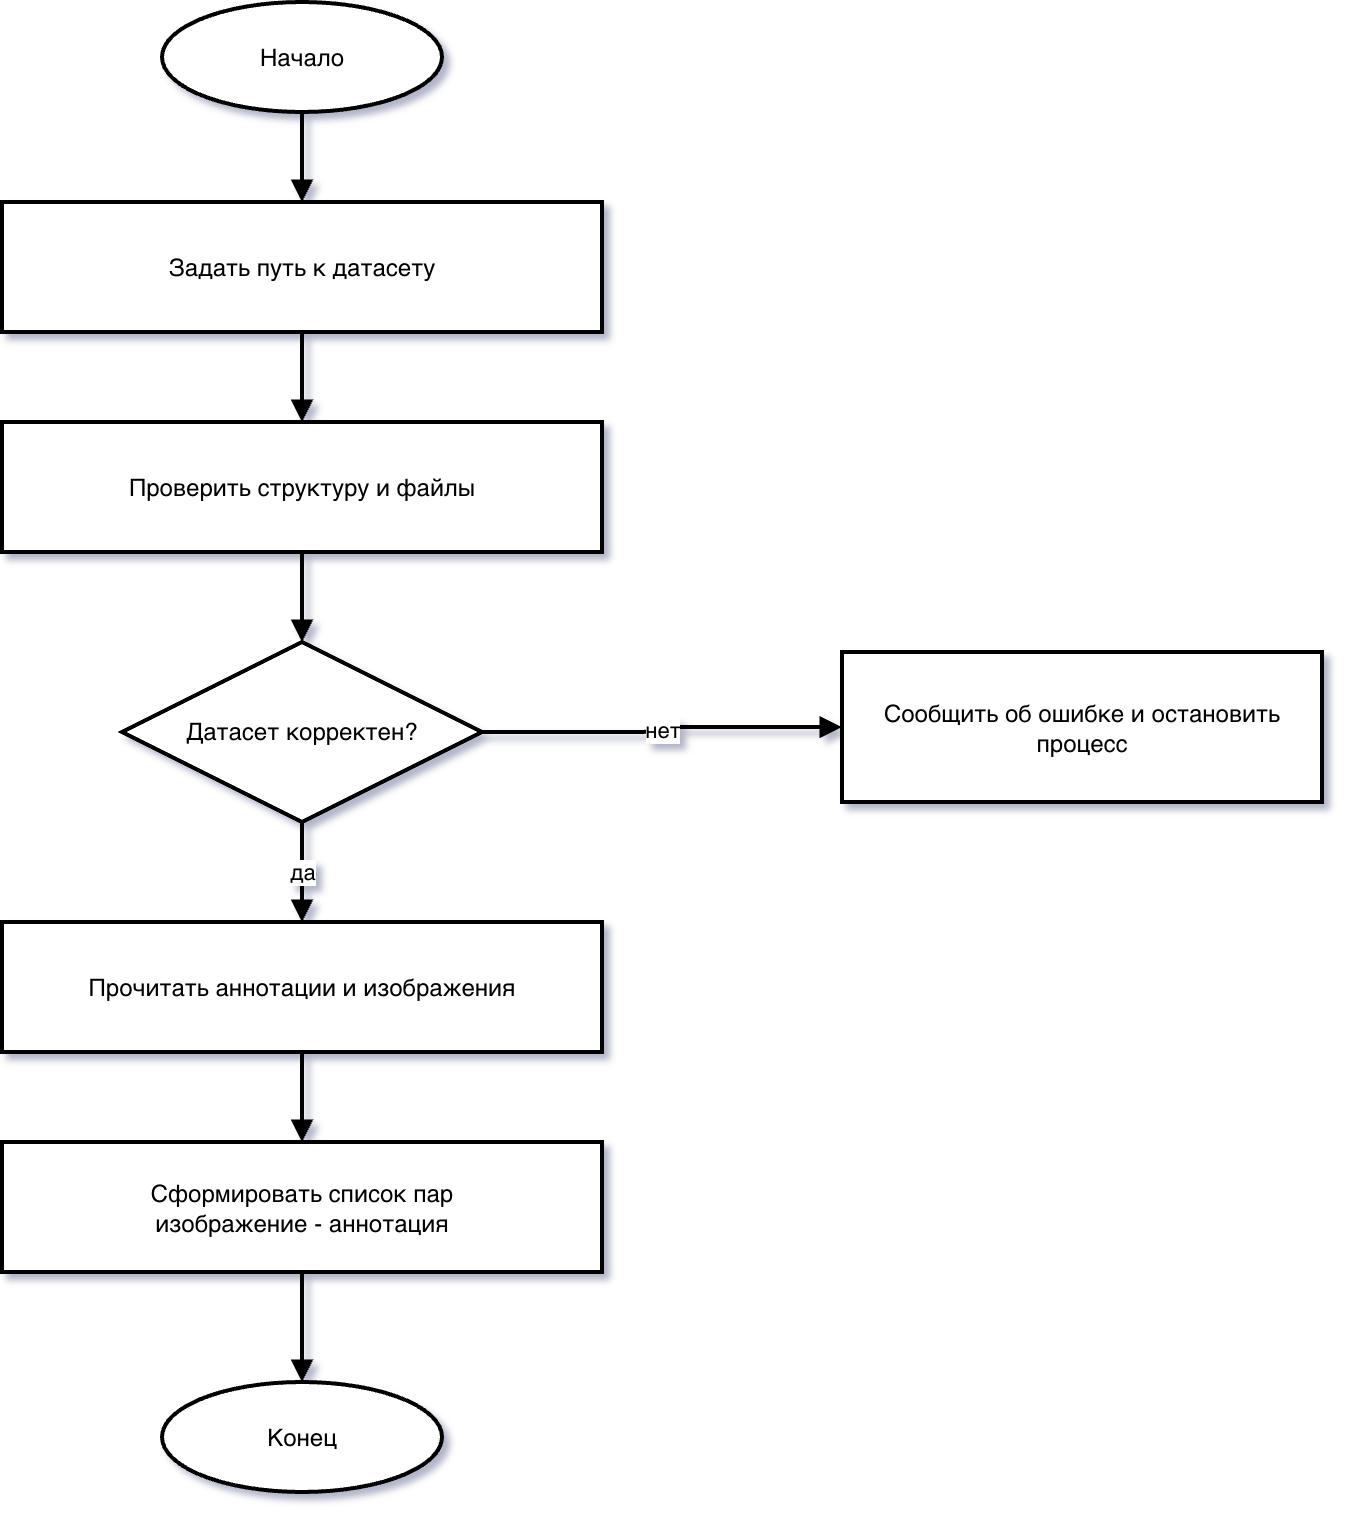
\includegraphics[width=\linewidth]{images/Загрузка_датасета.drawio.png}
\captionof{figure}{Блок-схема загрузки датасета}
\label{fig:dataset_loading}
\end{figure}

\subsubsection{Предобработка изображений}

\begin{figure}[H]
    \centering
    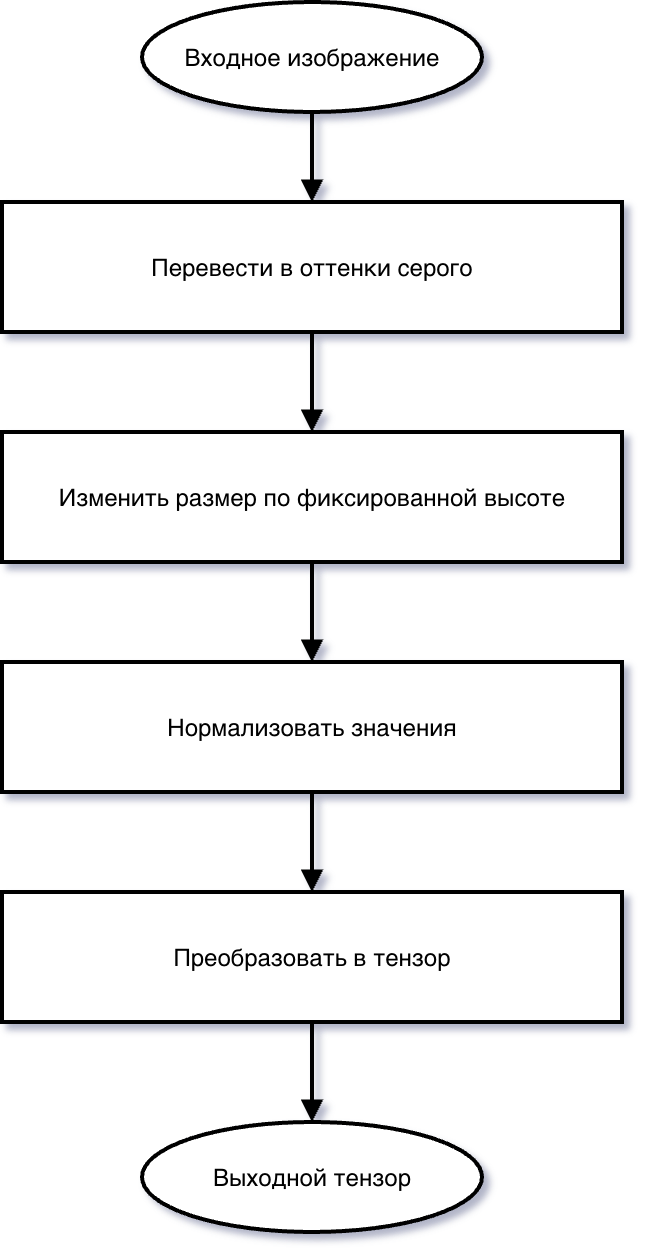
\includegraphics[width=\textwidth,height=0.8\textheight,keepaspectratio]{images/Предобработка.drawio.png}
    \captionof{figure}{Блок-схема предобработки изображений}
    \label{fig:image_preprocessing}
\end{figure}

\subsubsection{Обучение CRNN}
\begin{figure}[H]
    \centering
    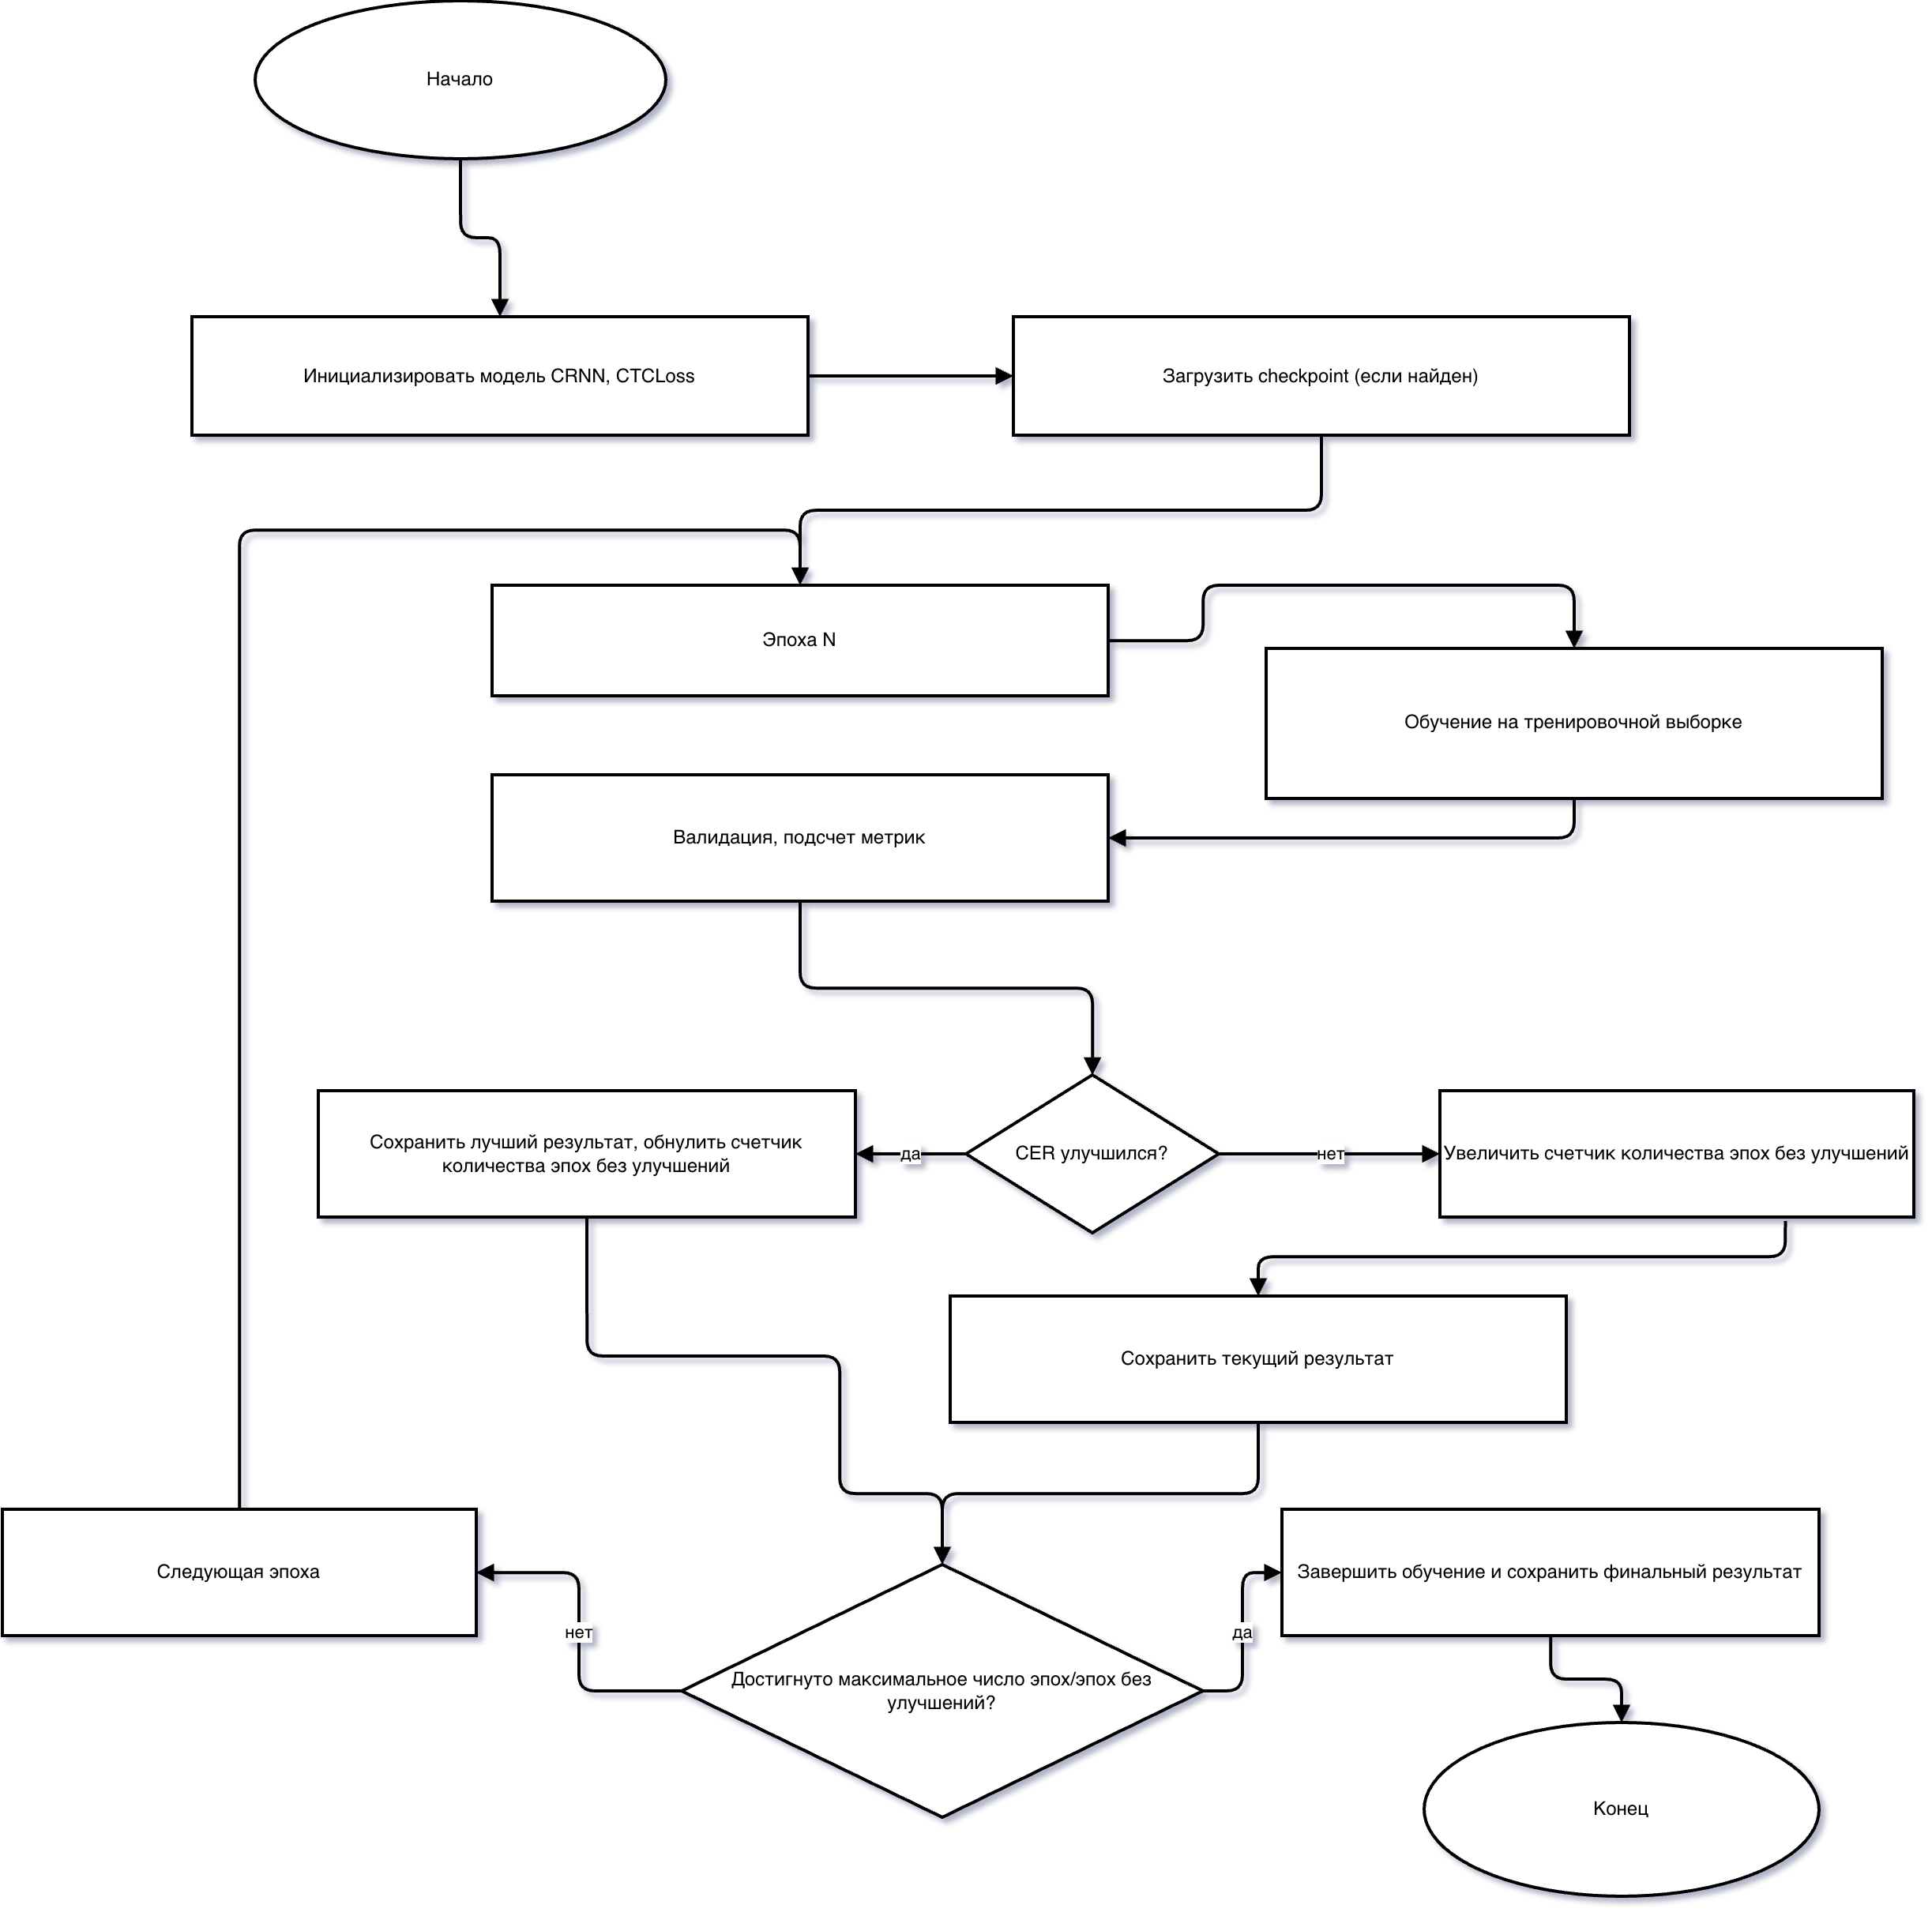
\includegraphics[width=\linewidth]{images/Обучение_CRNN.drawio.png}
    \captionof{figure}{Блок-схема обучения CRNN-модели}
    \label{fig:crnn_training}
\end{figure}

\subsubsection{Применение обученной модели к изображениям}
\begin{figure}[H]
    \centering
    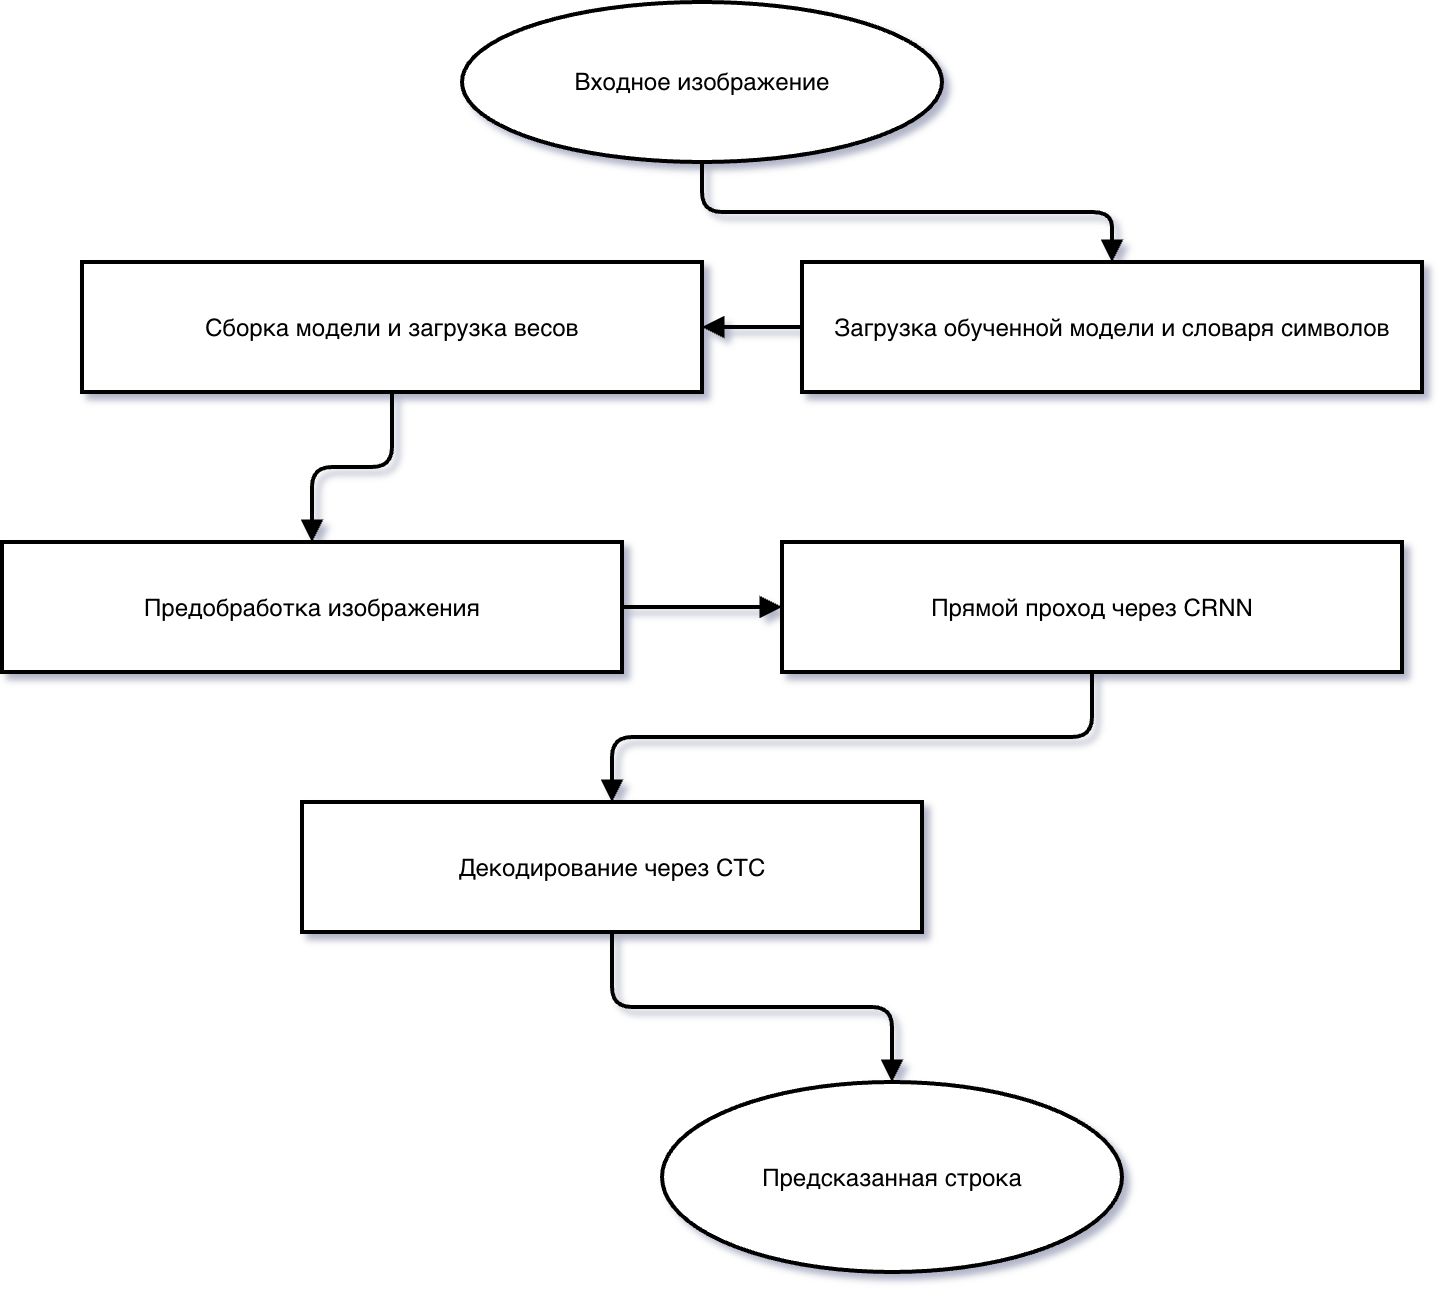
\includegraphics[width=\linewidth]{images/Инференс.drawio.png}
    \captionof{figure}{Блок-схема инференса с обученной CRNN-моделью}
    \label{fig:inference}
\end{figure}

\subsubsection{Постобработка распознанного текста}
\begin{figure}[H]
    \centering
    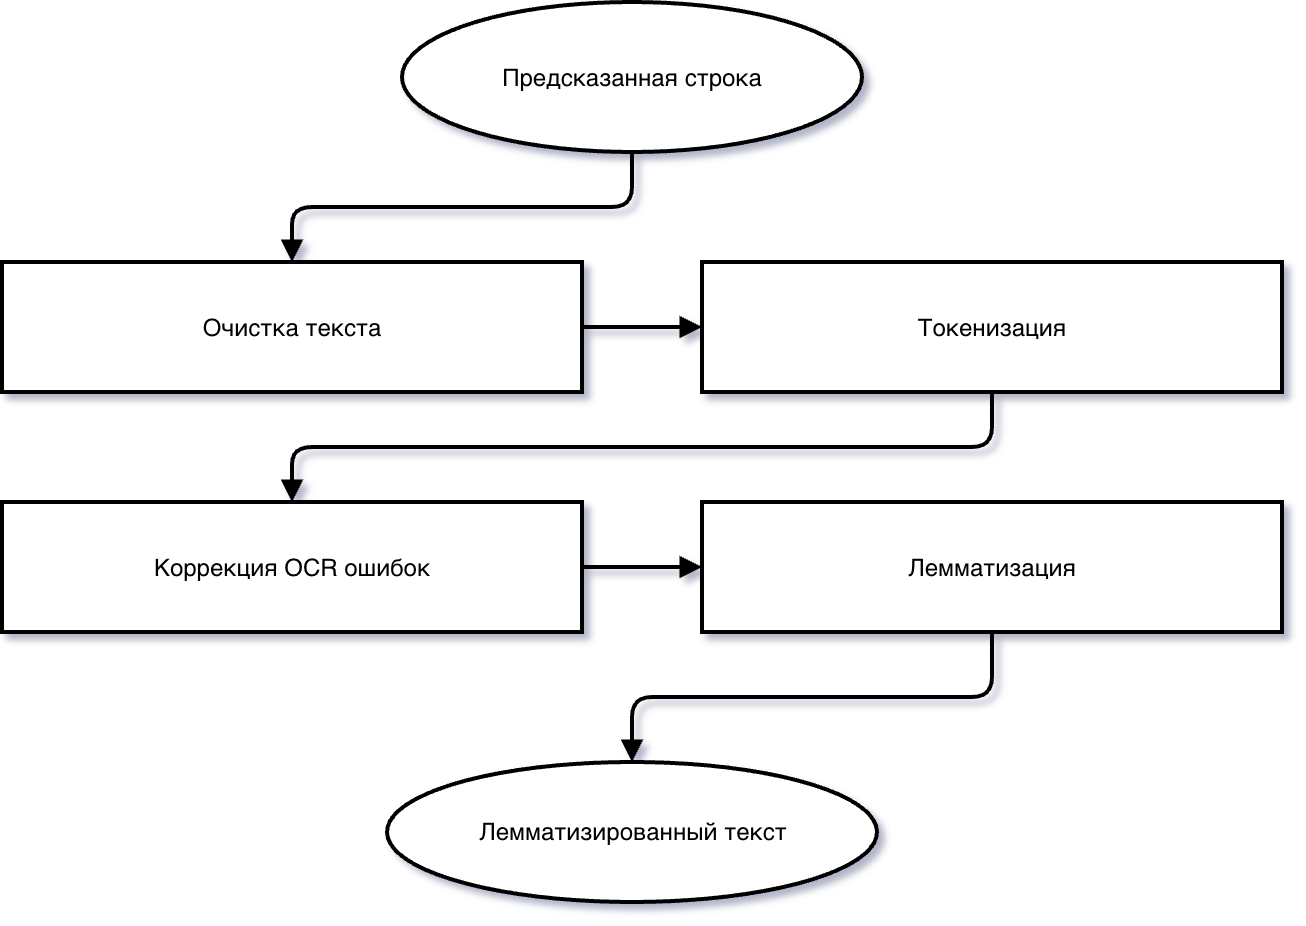
\includegraphics[width=\linewidth]{images/Постобработка.drawio.png}
    \captionof{figure}{Блок-схема постобработки распознанного текста}
    \label{fig:text_postprocessing}
\end{figure}

\subsubsection{Анализ эмоций}
\begin{figure}[H]
    \centering
    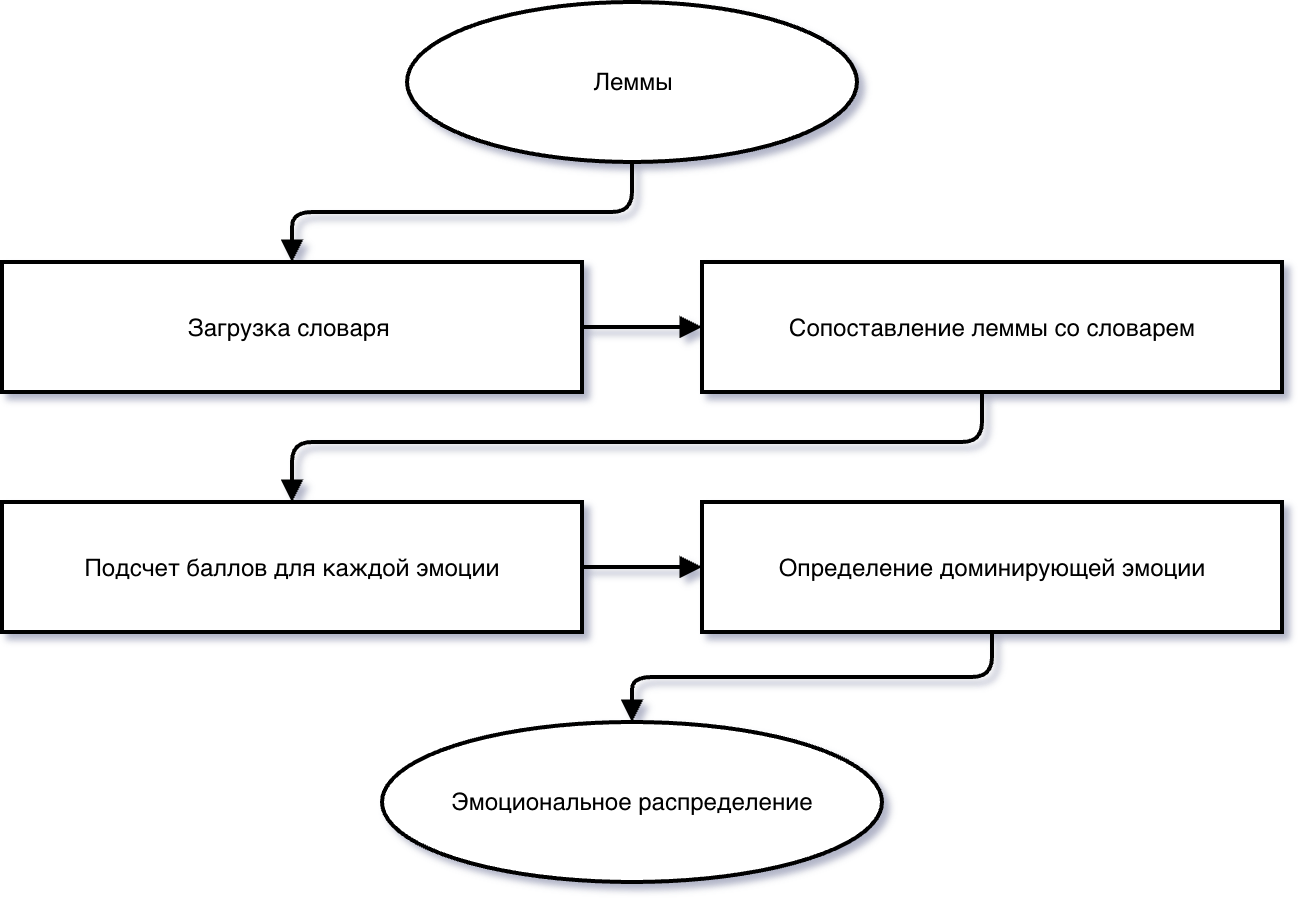
\includegraphics[width=\linewidth]{images/Анализ_эмоций.drawio.png}
    \captionof{figure}{Блок-схема анализа эмоций}
    \label{fig:emotion_analysis}
\end{figure}


\section{Рекомендации пользователю}

\begin{figure}[H]
    \centering
    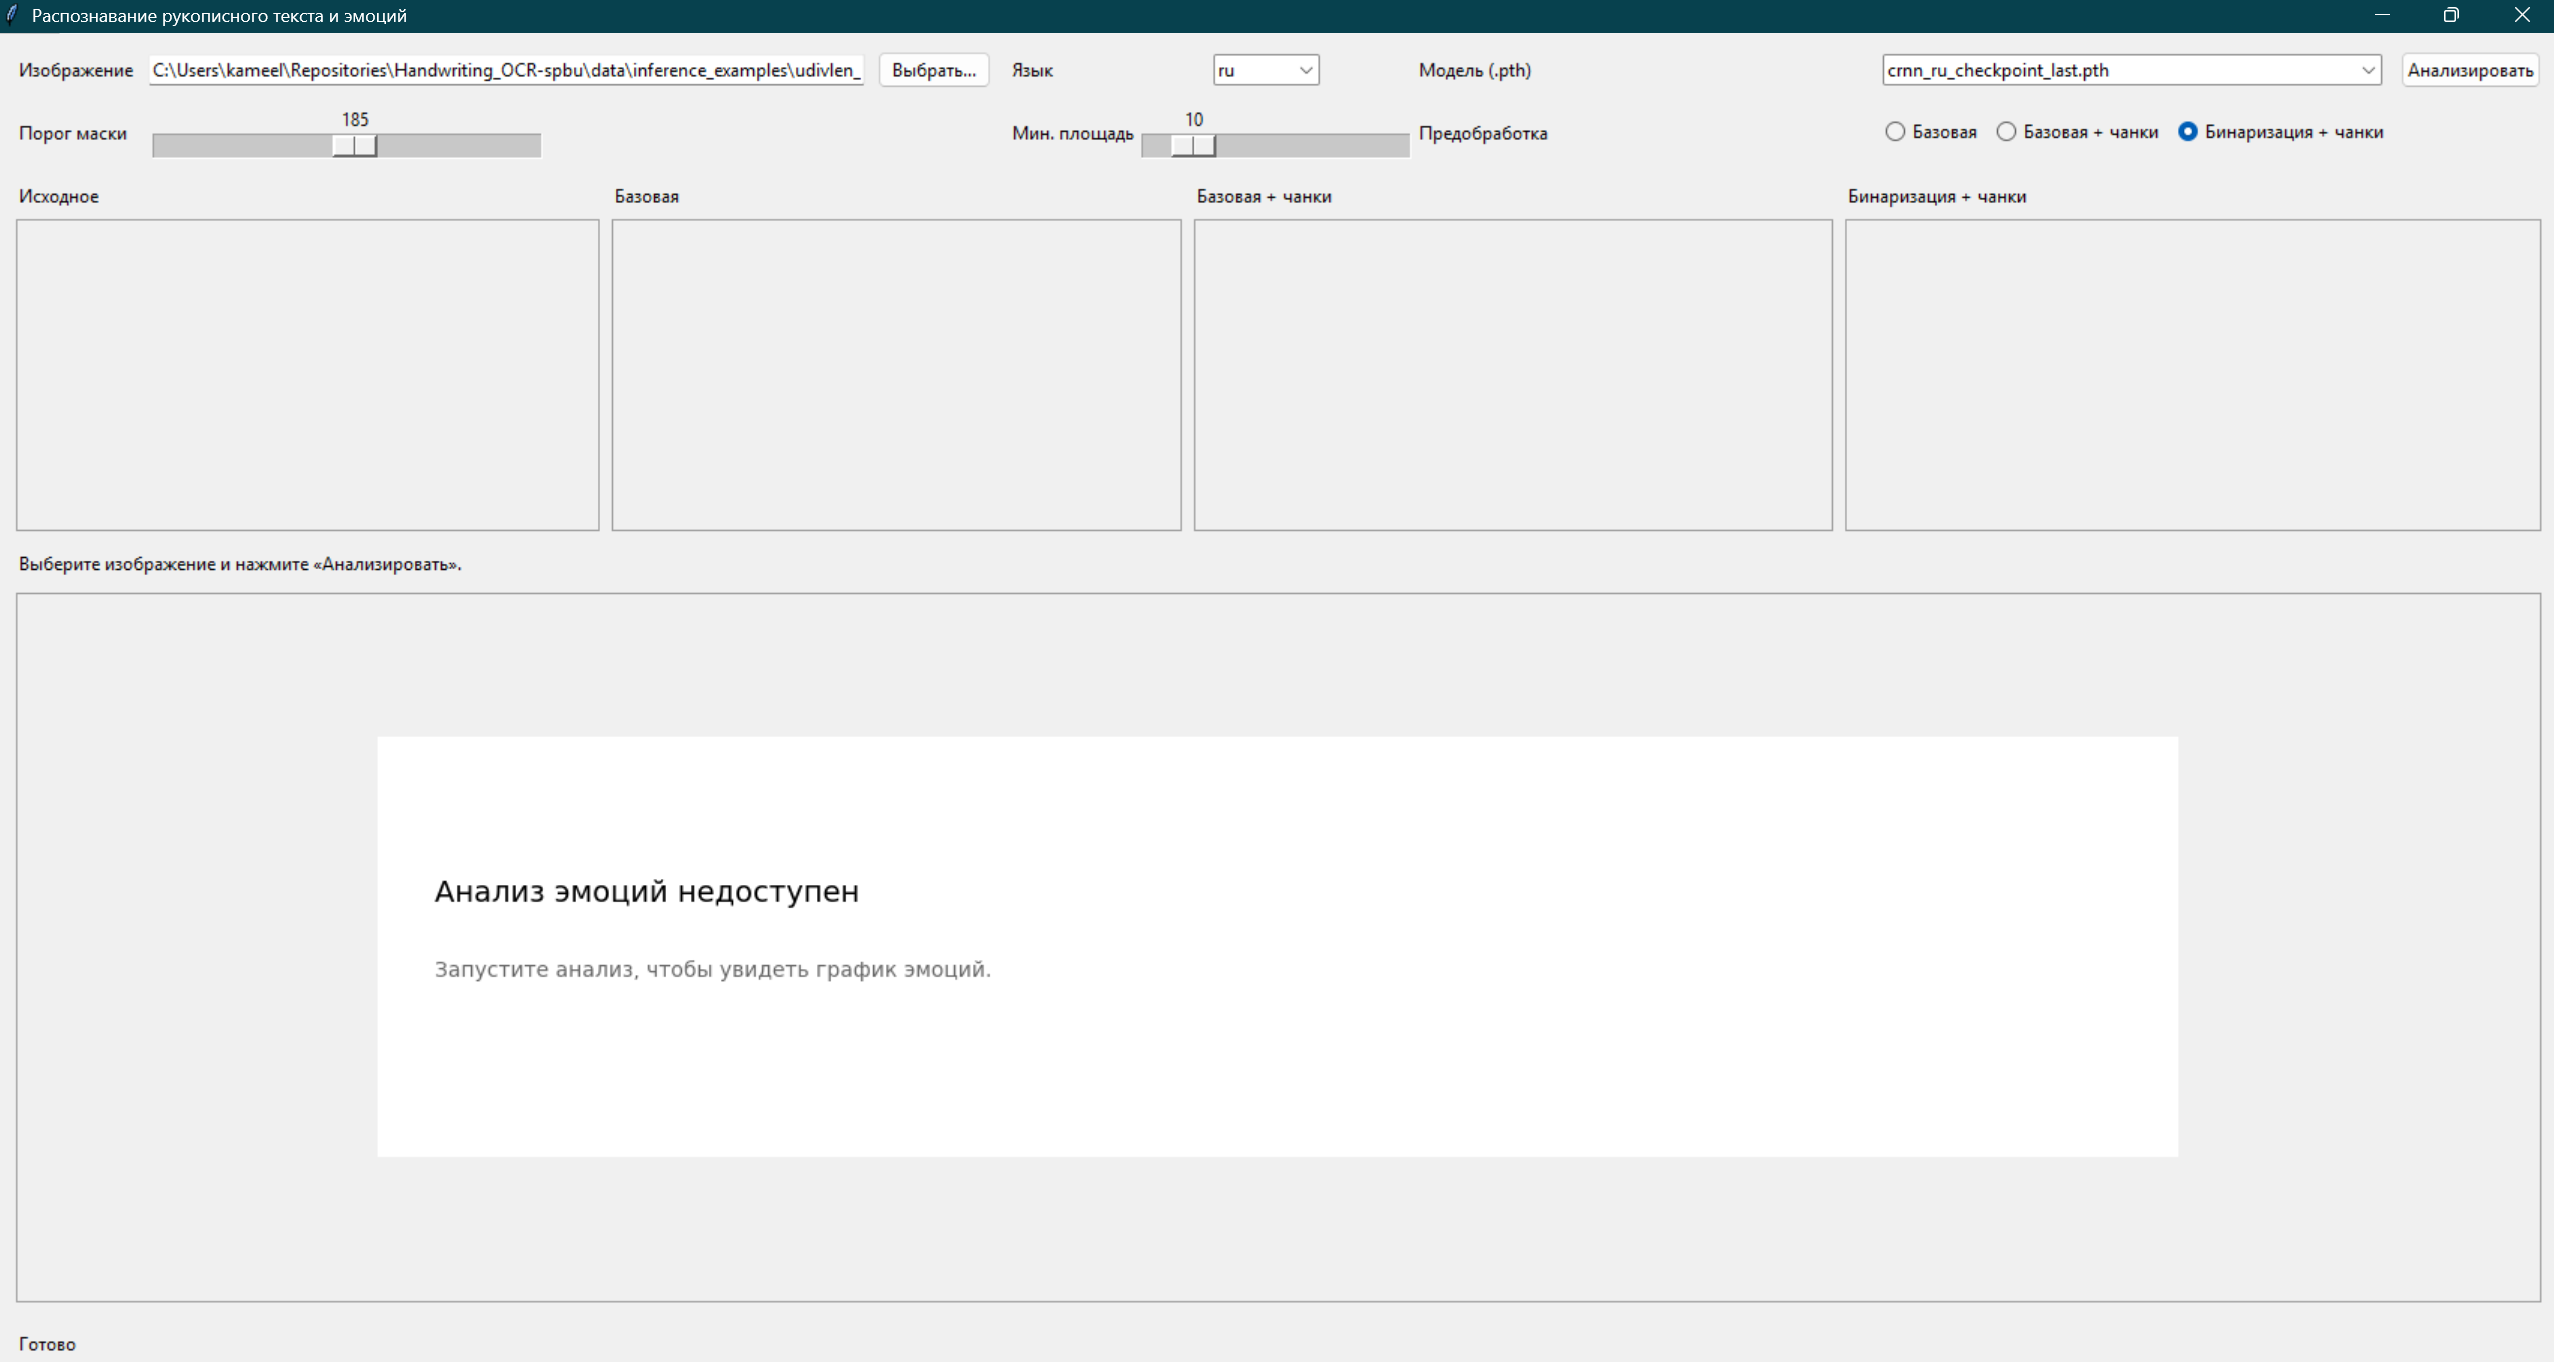
\includegraphics[width=\linewidth]{images/Рекомендации_пользователю_1.png}
    \captionof{figure}{Пользовательский интерфейс программы}
    \label{fig:user_guide}
\end{figure}
\subsection{Описание элементов интерфейса}

\begin{description}
    \item[Поле Изображение]
    Путь к изображению, которое будет передано на распознавание. Для выбора файла
    следует нажать кнопку \texttt{Выбрать}. Если изображение не выбрано или путь указан
    неверно, программа не сможет выполнить анализ и выведет сообщение об ошибке.

    \item[Поле Язык]
    Язык распознаваемого рукописного текста. Для русскоязычных изображений необходимо
    выбирать значение \texttt{ru}, для англоязычных --- \texttt{en}. От выбранного языка
    зависит выбор подходящей модели распознавания и возможность дальнейшего анализа
    эмоциональной окраски.

    \item[Поле Модель]
    Файл сохраненного состояния модели, который будет использован для распознавания.
    Рекомендуется выбирать checkpoint, соответствующий выбранному языку. Для русского
    текста следует использовать русскую модель, для английского --- английскую.
    Неверно выбранный checkpoint может привести к ухудшению качества распознавания.

    \item[Кнопка Анализировать]
    Кнопка запускает полный цикл обработки: загрузку изображения, предобработку,
    распознавание текста, построение вариантов результата и, для русского текста,
    анализ эмоциональной окраски. Перед нажатием необходимо убедиться, что выбраны
    файл изображения, язык и checkpoint.

    \item[Параметр Порог маски]
    Порог бинаризации изображения. При увеличении значения больше пикселей будет
    относиться к фону, при уменьшении --- к рукописному тексту. Если текст на
    изображении плохо отделяется от бумаги, параметр можно изменить и повторно
    запустить анализ.

    \item[Параметр Минимальная площадь]
    Минимальный размер связной компоненты, которая считается значимой. Мелкие
    компоненты меньше указанного значения удаляются как шум. Если после обработки
    пропадают части букв, значение следует уменьшить. Если остается много мелких
    пятен, значение можно увеличить.

    \item[Переключатель Предобработка]
    Вариант распознавания, по которому строится график эмоционального анализа:
    \begin{itemize}
        \item \texttt{Базовая} --- распознавание изображения целиком;
        \item \texttt{Базовая + чанки} --- распознавание с дополнительной сегментацией;
        \item \texttt{Бинаризация + чанки} --- бинаризация и сегментация перед распознаванием.
    \end{itemize}
    Рекомендуется сравнивать все три варианта, так как качество может зависеть от
    конкретного изображения.
\end{description}

\subsection{Интерпретация результатов}

\begin{itemize}
    \item Область \texttt{Исходное} показывает исходное изображение, выбранное пользователем.
    \item Области \texttt{Базовая}, \texttt{Базовая + чанки} и
    \texttt{Thresholded + чанки} отображают результаты разных способов обработки
    и распознавания.
    \item По этим областям можно визуально оценить, какой вариант лучше сохранил
    структуру рукописного текста.
    \item Нижняя часть окна предназначена для вывода текстового результата и графика
    эмоциональной окраски.
    \item До запуска анализа в этой области отображается сообщение о том, что анализ
    эмоций недоступен.
    \item После обработки изображения программа показывает распознанный текст,
    исправленный текст, доминирующую эмоцию и распределение по эмоциональным категориям,
    если анализ применим к выбранному языку.
\end{itemize}

\subsection{Рекомендации по использованию}

\begin{itemize}
    \item Для получения более качественного результата рекомендуется использовать
    изображения с четким рукописным текстом, без сильного размытия, бликов, резких
    теней и лишних объектов на фоне.
    \item Желательно, чтобы строка текста была расположена горизонтально, а буквы
    были достаточно крупными и контрастными относительно бумаги.
    \item Если результат распознавания оказался неточным, рекомендуется попробовать
    другой вариант обработки, изменить параметры \texttt{Порог маски} и
    \texttt{Минимальная площадь}, а затем повторно нажать \texttt{Анализировать}.
    \item Для длинных строк и фраз часто полезны варианты с сегментацией, так как
    программа распознает отдельные фрагменты изображения и затем объединяет результат.
    \item Анализ эмоциональной окраски предназначен прежде всего для русского текста.
    Он работает надежнее, если во входном изображении содержится не одно короткое слово,
    а фраза из нескольких содержательных слов.
    \item При слишком коротком тексте или большом количестве ошибок OCR эмоциональный
    анализ может не выявить доминирующую эмоцию.
    \item Для завершения работы с программой достаточно закрыть окно приложения
    стандартной кнопкой закрытия окна.
\end{itemize}

\section{Рекомендации программисту и дополнительные сведения о ПО}

\subsection{Структура и зависимости проекта}

\begin{itemize}
    \item Программа написана на языке Python с использованием библиотеки PyTorch для нейросетевой части, NumPy для обработки данных и других вспомогательных библиотек.
    \item Исходный код блоков по обучению и инференсу CRNN-модели, а также предобработки изображений и анализа эмоций, находится в папке \texttt{src}. Рекомендуется ознакомиться с кодом, чтобы понять структуру программы и логику работы каждого компонента.
    \item Для удобства навигации по коду создан Jupyter Notebook \texttt{train.ipynb}, который содержит код для обучения модели и может быть запущен в среде Jupyter.
    \item При запуске программы необходимо убедиться, что все зависимости установлены, и что выбранные checkpoint-файлы соответствуют языку распознаваемого текста. Рекомендуется использовать предоставленные checkpoint-файлы, так как они были обучены на соответствующих датасетах и обеспечивают оптимальное качество распознавания.
\end{itemize}

\subsection{Системные требования}

Для запуска программы необходимо следующее:
\begin{itemize}
    \item Python 3.8 или выше;
    \item достаточный объем оперативной памяти (рекомендуется 16 ГБ и выше);
    \item видеокарта для GPU-инференса (опционально, но рекомендуется);
    \item виртуальное окружение для управления зависимостями.
\end{itemize}

\subsection{Проверка совместимости}

Работоспособность инференса была проверена на следующих конфигурациях:

\begin{table}[H]
\caption{Протестированные конфигурации систем}
\label{tab:system_configs}
\centering
\footnotesize
\setlength{\tabcolsep}{3pt}
\renewcommand{\arraystretch}{1.15}
\begin{tabularx}{\linewidth}{|
>{\raggedright\arraybackslash}p{1.7cm}|
>{\centering\arraybackslash}p{1.0cm}|
>{\centering\arraybackslash}p{2.0cm}|
>{\raggedright\arraybackslash}X|
>{\centering\arraybackslash}p{1.4cm}|
>{\raggedright\arraybackslash}X|}
\hline
\textbf{ОС} & \textbf{Python} & \textbf{PyTorch} & \textbf{Процессор} & \textbf{Объем ОЗУ} & \textbf{Видеокарта} \\
\hline
Windows 11 & 3.14 & 2.11 & AMD Ryzen 7 7840H & 16 ГБ & AMD Radeon 780M \\
\hline
Windows 11 & 3.14 & 2.11 CUDA 12.8 & Ryzen 5 8400F & 32 ГБ & NVIDIA GeForce RTX 3060 12GB \\
\hline
macOS 26.2 & 3.14 & 2.11 & Apple M1 Pro & 16 ГБ & 14-core GPU \\
\hline
\end{tabularx}
\end{table}

На всех перечисленных системах вывод модели работает корректно, что подтверждает универсальность и стабильность разработанной программы.

\subsection{Рекомендации по использованию GPU и CPU}

\subsubsection{Вывод модели}

Запуск вывода модели на графическом процессоре (GPU) значительно ускоряет процесс распознавания. Запуск на центральном процессоре (CPU) также возможен, но может занять значительно больше времени, особенно для более сложных изображений и длинных строк текста.

\subsubsection{Обучение}

Обучение производилось на видеокарте NVIDIA GeForce RTX 3060 12GB и заняло примерно 2 часа для достижения приемлемого качества распознавания. Рекомендуется использовать аналогичное или более мощное оборудование для обучения модели.

Перед запуском обучения необходимо:
\begin{itemize}
    \item проверить установку последних версий драйверов видеокарты;
    \item убедиться, что версия PyTorch поддерживает CUDA (если планируется использовать GPU с поддержкой CUDA).
\end{itemize}

\textbf{Внимание:} запуск обучения на центральном процессоре (CPU) не рекомендуется, так как это может занять от нескольких часов до нескольких дней в зависимости от объема данных и сложности модели.



\section{Контрольный пример}

В качестве контрольного примера используется файл \texttt{happy.jpg} из директории
\texttt{data/inference\_examples}. На изображении приведена фраза на русском языке.
Для запуска пользовательского интерфейса используется файл
\texttt{ocr\_emotion\_ui.py}. После запуска открывается окно приложения
\texttt{Распознавание рукописного текста и эмоций}, в котором пользователь выбирает изображение,
язык распознавания, checkpoint модели и параметры предварительной обработки.

\begin{figure}[H]
    \centering
    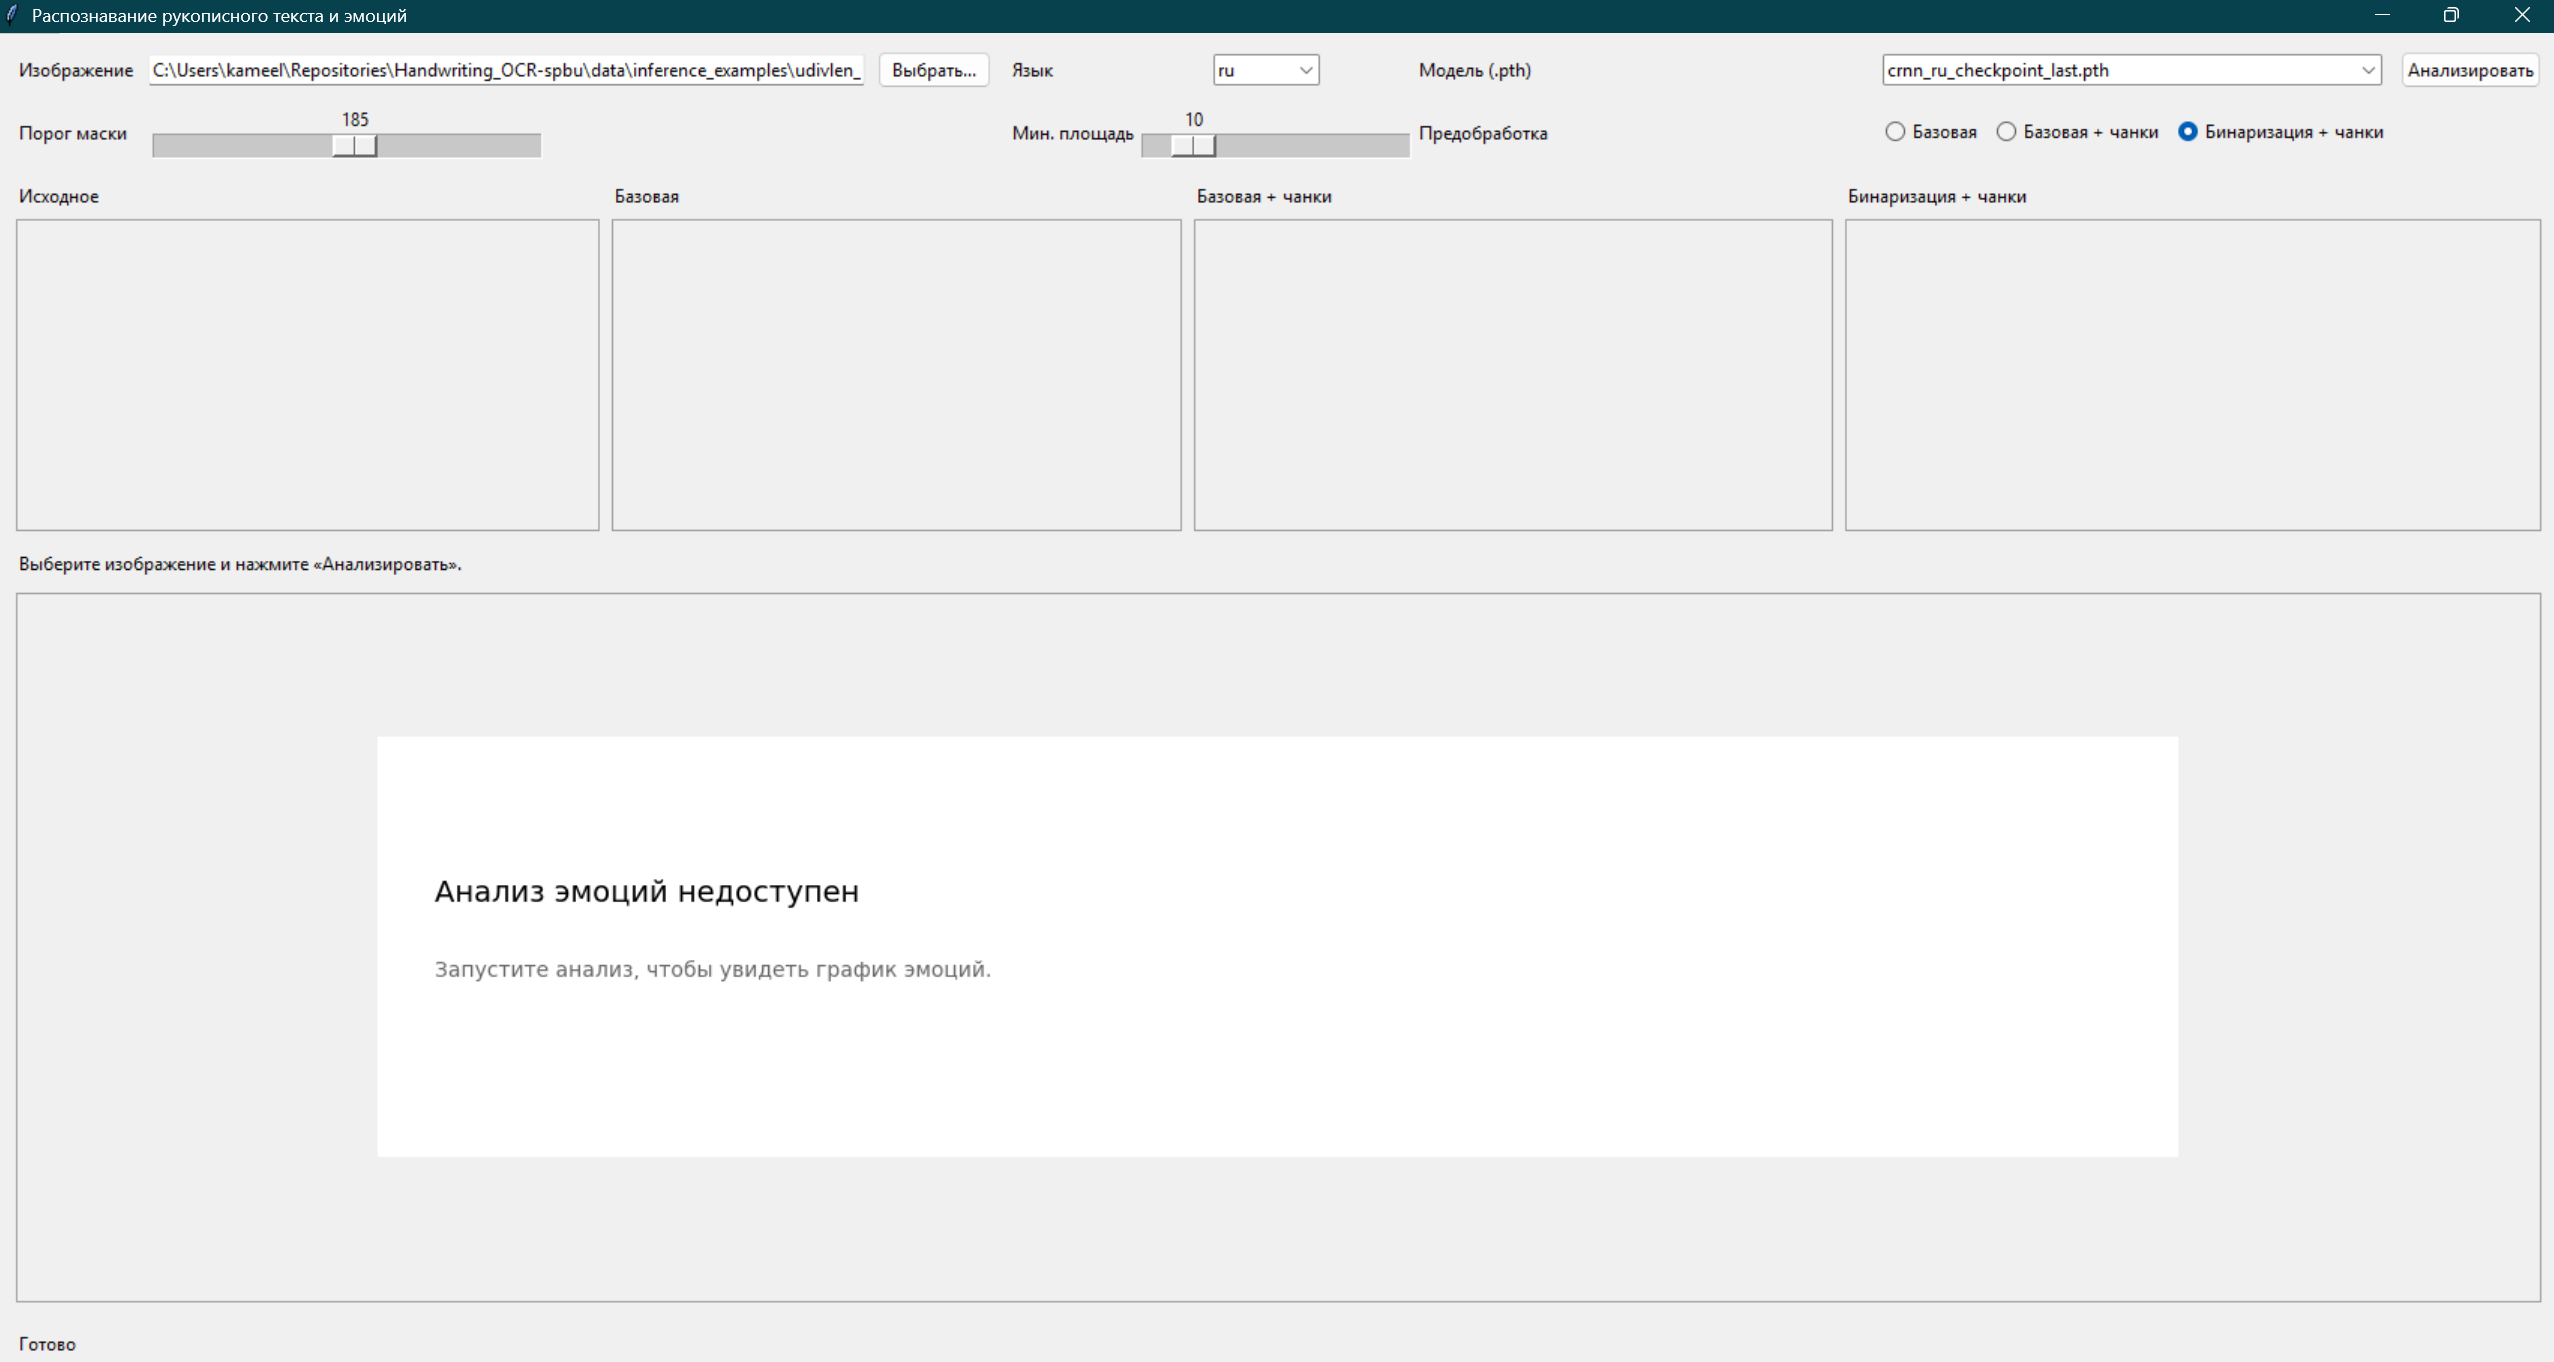
\includegraphics[width=\linewidth]{images/Контрольный_1.png}
    \captionof{figure}{Пользовательский интерфейс программы}
    \label{fig:user_interface}
\end{figure}

В верхней части окна расположены следующие элементы:
\begin{itemize}
    \item \textbf{Изображение} --- путь к изображению с рукописным текстом. Кнопка
    \textbf{Выбрать} позволяет выбрать файл через стандартное окно выбора.
    \item \textbf{Язык} --- язык распознавания.
\item \textbf{Модель} --- файл сохраненного состояния модели, используемый
    для распознавания.
    \item \textbf{Порог маски} --- порог бинаризации.
    \item \textbf{Минимальная площадь} --- минимальная площадь компоненты, которая не считается шумом.
    \item \textbf{Предобработка} --- вариант распознавания, по которому строится график эмоционального анализа.
    \item \textbf{Анализировать} --- запуск полного цикла обработки изображения.
\end{itemize}

Для примера выбраны следующие параметры:
\begin{itemize}
    \item контрольная точка \texttt{crnn\_checkpoint\_last\_ru\_bs24\_512x3\_final.pth};
    \item \texttt{Порог маски = 160};
    \item \texttt{Минимальная площадь = 80};
    \item источник графика --- \texttt{Базовая + чанки}.
\end{itemize}

\begin{figure}[H]
    \centering
    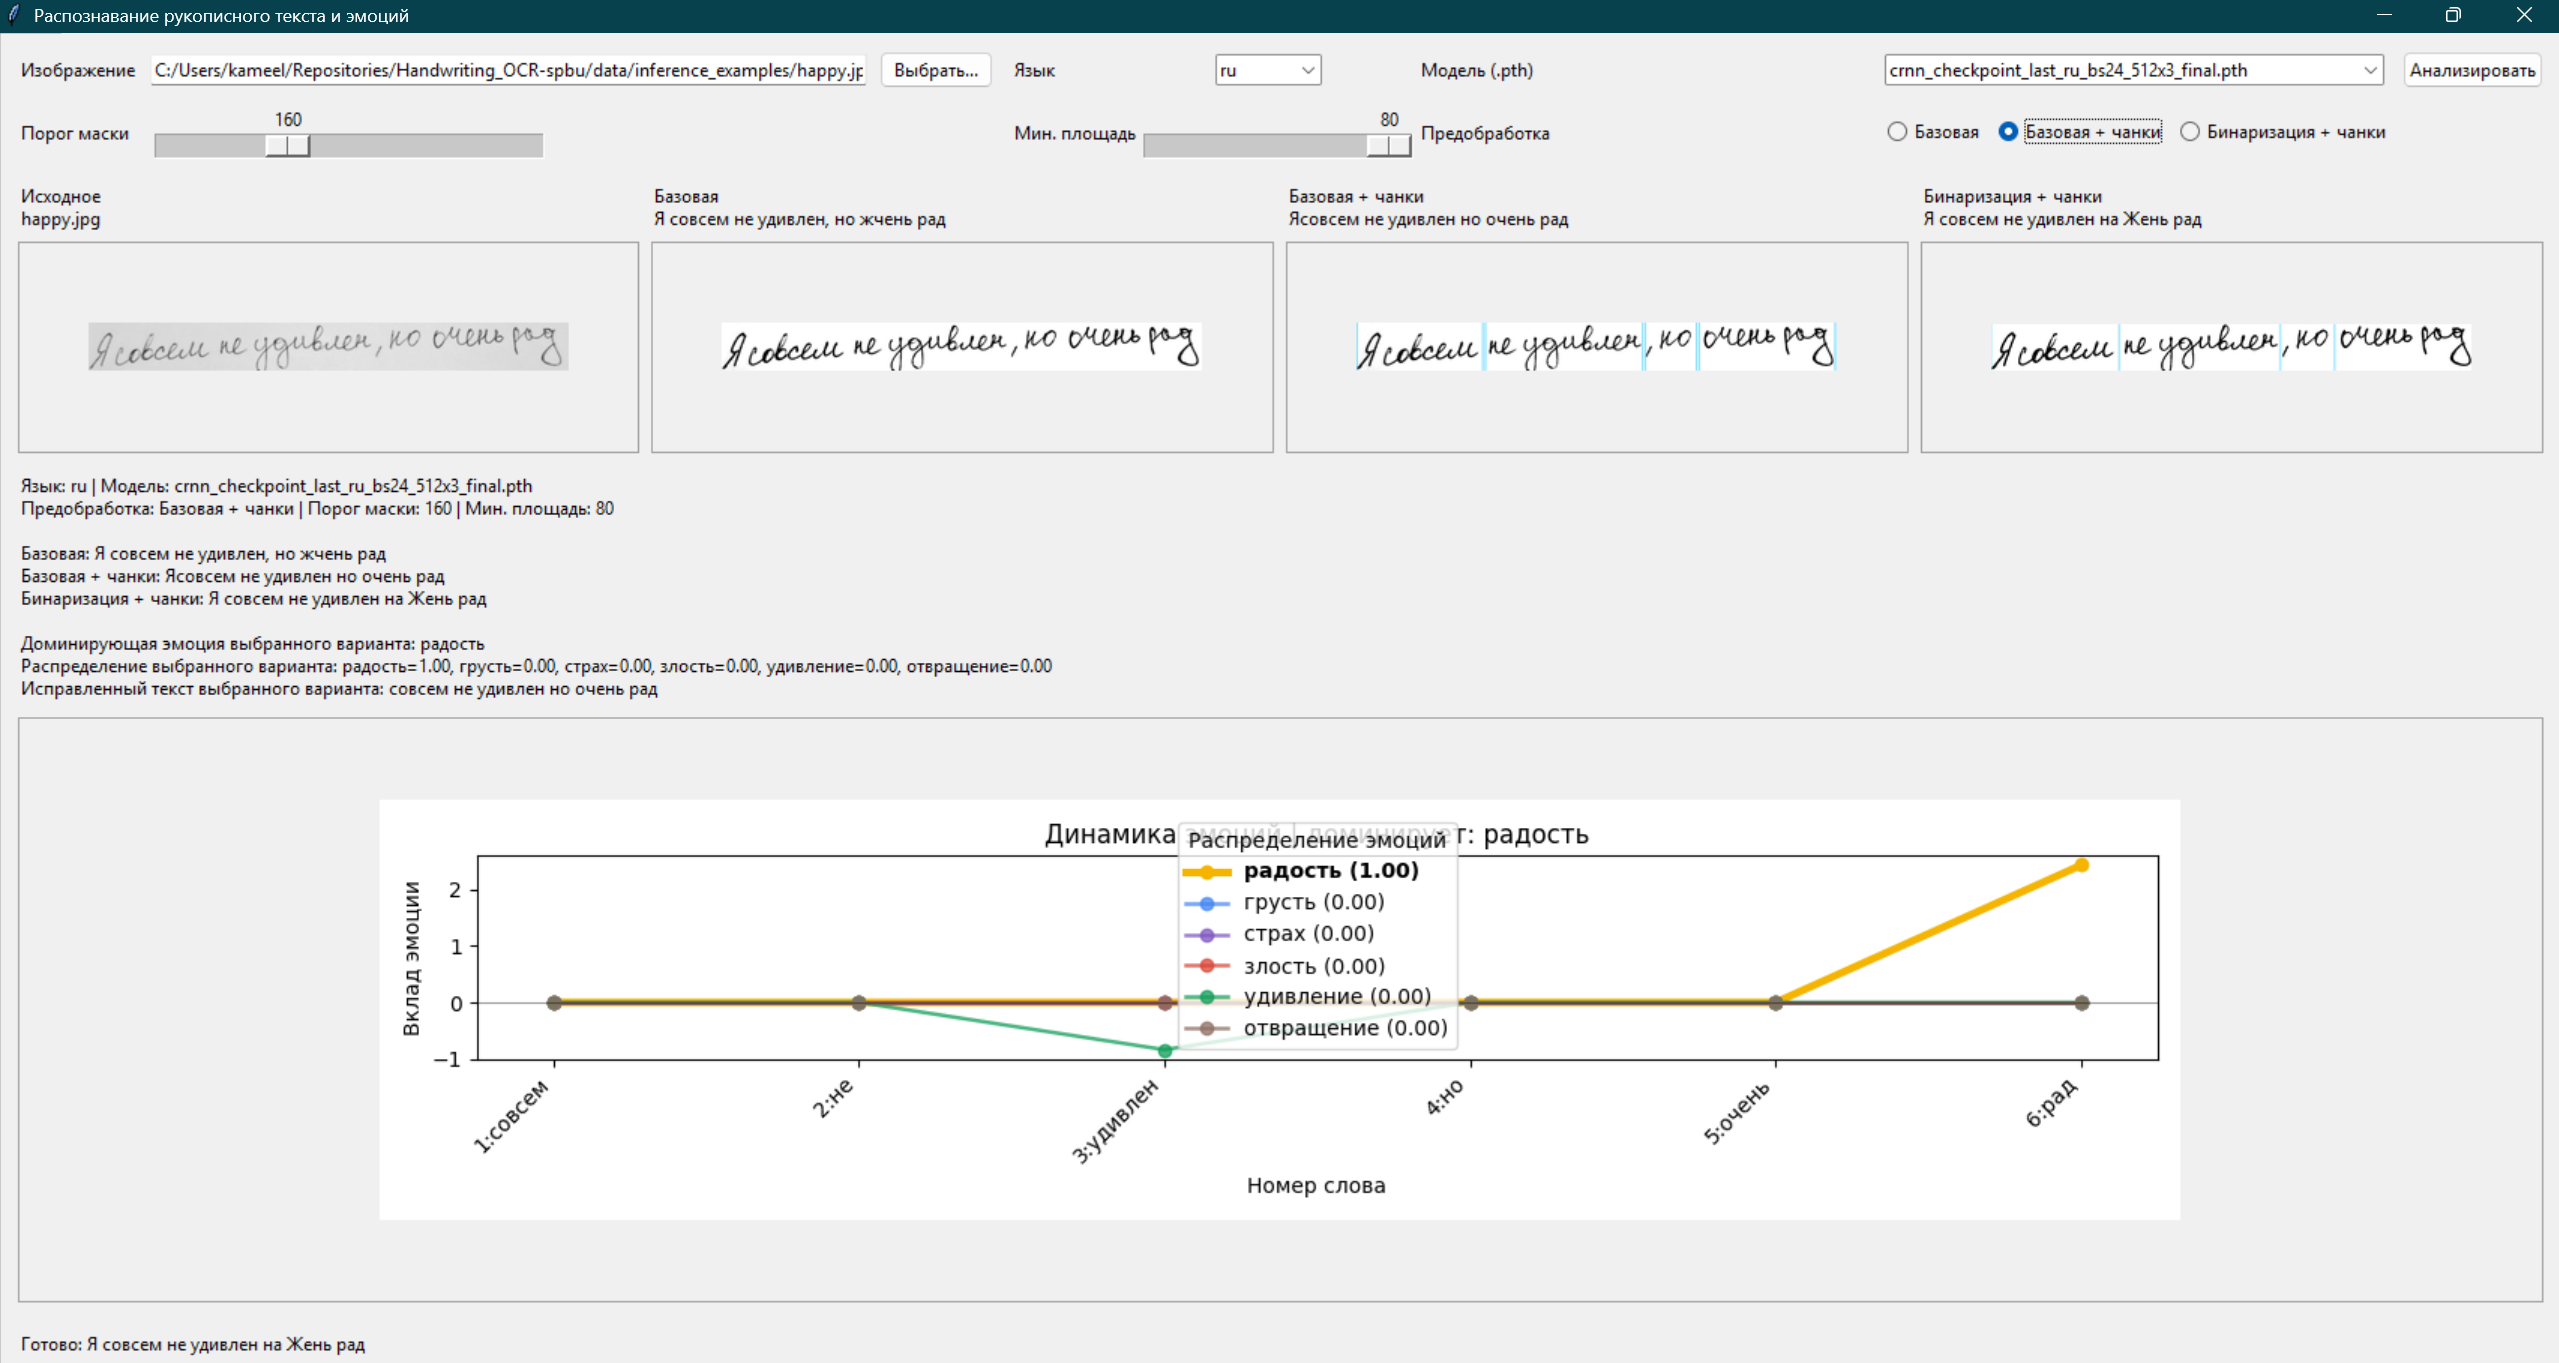
\includegraphics[width=\linewidth]{images/Контрольный_2.png}
    \captionof{figure}{Результат распознавания и анализа эмоций для контрольного примера}
    \label{fig:control_example_result}
\end{figure}

После нажатия кнопки \textbf{Анализировать} программа отображает исходное изображение и
три варианта распознавания:
\begin{itemize}
    \item \textbf{Базовая} --- \texttt{Я совсем не удивлен, но жчень рад};
    \item \textbf{Базовая + чанки} --- \texttt{Ясовсем не удивлен но очень рад};
    \item \textbf{Thresholded + чанки} --- \texttt{Я совсем не удивлен на Жень рад}.
\end{itemize}

Несмотря на ошибки распознавания отдельных символов, модуль постобработки
исправляет выбранный текст до фразы \texttt{совсем не удивлен но очень рад}. Это
показывает, что коррекция ошибок распознавания текста помогает подготовить результат распознавания
к дальнейшему анализу эмоциональной окраски.

В результате анализа эмоций программа определяет доминирующую эмоцию
\texttt{радость}. Распределение эмоций для выбранного варианта имеет вид:
\texttt{радость = 1.00}, \texttt{грусть = 0.00}, \texttt{страх = 0.00},
\texttt{злость = 0.00}, \texttt{удивление = -1.00}, \texttt{отвращение = 0.00}.
Это соответствует смыслу исходной фразы, так как ключевым эмоционально окрашенным
словом является \texttt{рад}.

На графике эмоционального анализа по оси \texttt{Номер слова} отображаются слова
исправленного текста, а по вертикальной оси --- вклад каждого слова в эмоциональные
категории. Слово \texttt{удивлен} находится под действием отрицания \texttt{не},
поэтому итоговая доминирующая эмоция не становится удивлением. Основной
положительный вклад вносит слово \texttt{рад}, из-за чего выбранной эмоцией
становится радость.


\section{Исследование и разработка}
 
\subsection{Обзор литературы}

В ходе подготовки работы был проведён разбор некоторых публикаций, посвященных распознаванию
рукописного текста и анализу эмоций в тексте. Общее понимание о современных подходах к OCR и
к истории их развития дает статья Handwritten Text Recognition: A survey. \cite{survey2023}.

Классические гибридные подходы, сочетающие HMM/ANN и признаки ручной разработки, описаны в ряде
статей и остаются релевантными для задач распознавания текстов с невариативным почерком \cite{hybridhmm2010}.
Наиболее совершенным подходом к распознаванию рукописных текстов являются
методы, использующие многомерные рекуррентные сети (MD-RNN) и их модификации. Данные алгоритмы
имеют высокую точность засчет применения методов, опирающихся на контекст.

Проводить обучение без выравнивания можно благодаря алгоритму CTC, который позволяет тренировать
модели по парам «изображение—строка» без посимвольной разметки и широко применяется в архитектурах типа CRNN
\cite{ctc2006}. Проблемы сегментации строк и слов подробно рассматриваются в работах по предобработке документов и
выделению текстовых строк из сложных сцен и рукописных страниц \cite{segmentation2009}.

Наиболее совершенные подходы представлены в исследования по конструированию эффективных end-to-end архитектур
и трансформеров для OCR. Данные методы демонстрируют рост точности на сложных датасетах, но отмечают возросшие
требования к ресурсам и данным \cite{e2eneural2018,survey2023}.

Для анализа эмоциональной окраски текста обзор показал два основных подхода: лексиконные методы
и методы на основе машинного обучения. Лексиконные подходы опираются на зараннее составленные
словари (например, ANEW и последующие ресурсы) и дают прозрачные результаты при наличии
коррекции ошибок OCR \cite{anew1999,norms2013,ratings2018}. Более сложные ML-подходы используют
контекстные признаки и нейросетевые модели для учёта синтаксиса и негативных конструкций, что
повышает точность, но требует дополнительных ресурсов \cite{semanticemotion2019,rulesemotion2014}.

Выводы обзора легли в основу выбора архитектуры CRNN с CTC для основной OCR-пайплайна и лексиконного
подхода с коррекцией ошибок для анализа эмоций в данном проекте. 

\subsection{Сравнение подходов к распознаванию рукописного текста}

В ходе изучения предметной области были рассмотрены различные варианты реализации
функционала распознавания рукописного текста и анализа эмоций. Были изучены следующие
подходы к решению задачи по распознаванию текста с изображений:

\begin{table}[H]
\caption{Сравнение подходов к распознаванию рукописного текста}
\label{tab:approaches_comparison}
\centering
\small
\renewcommand{\arraystretch}{1.3}
\begin{tabularx}{\linewidth}{|
>{\raggedright\arraybackslash}X|
>{\raggedright\arraybackslash}X|
>{\raggedright\arraybackslash}X|}
\hline
\textbf{Подход} & \textbf{Преимущества} & \textbf{Недостатки} \\
\hline
Традиционные методы (например, метод опорных векторов (SVM), скрытые марковские модели (HMM) \cite{hybridhmm2010}) & 
Быстрое обучение на небольших данных & 
Низкая точность на сложных рукописных текстах \\
\hline
Сверточно-рекуррентная нейросеть (CRNN) \cite{ctc2006} & 
Не требует посимвольной разметки, устойчив к разной длине строк & 
Требует больше данных и вычислительных ресурсов, чувствителен к качеству предобработки \\
\hline
Модели на основе трансформеров (например, TrOCR \cite{e2eneural2018}) &
Высокая точность, особенно на сложных изображениях &
Очень требовательны к ресурсам, сложны в обучении, могут переобучаться на небольших наборах данных. \\
\hline
\end{tabularx}
\end{table}

На основе проведённого анализа была выбрана архитектура CRNN \cite{ctc2006}, так как она
обеспечивает оптимальный баланс между точностью распознавания и требуемыми
вычислительными ресурсами, что подтверждается современными обзорами в данной области \cite{survey2023}.


\subsection{Выбор данных для обучения модели}

В качестве первой версии набора данных, на котором обучалась модель, была выбрана база данных рукописного текста IAM (IAM Handwriting
Database) \cite{marti2002iam, iamdb2002}. Этот набор данных содержит рукописный английский
текст с аннотациями, что позволяет эффективно обучать модель распознавать английский
рукописный текст. Особенностью этого набора данных является наличие большого количества строк текста,
что позволяет модели учиться на разнообразных примерах.

После успешного обучения модели на английском языке, было принято решение расширить функционал
и добавить поддержку русского языка. Для этого был выбран набор данных HKR (HKR Dataset) \cite{hkr2024}, который
содержит рукописный текст на русском и казахском языках. Этот набор данных является более сложным для
распознавания из-за особенностей формата изображений, но он предоставляет необходимые данные
для обучения модели на русском языке.

\begin{figure}[H]
    \centering
    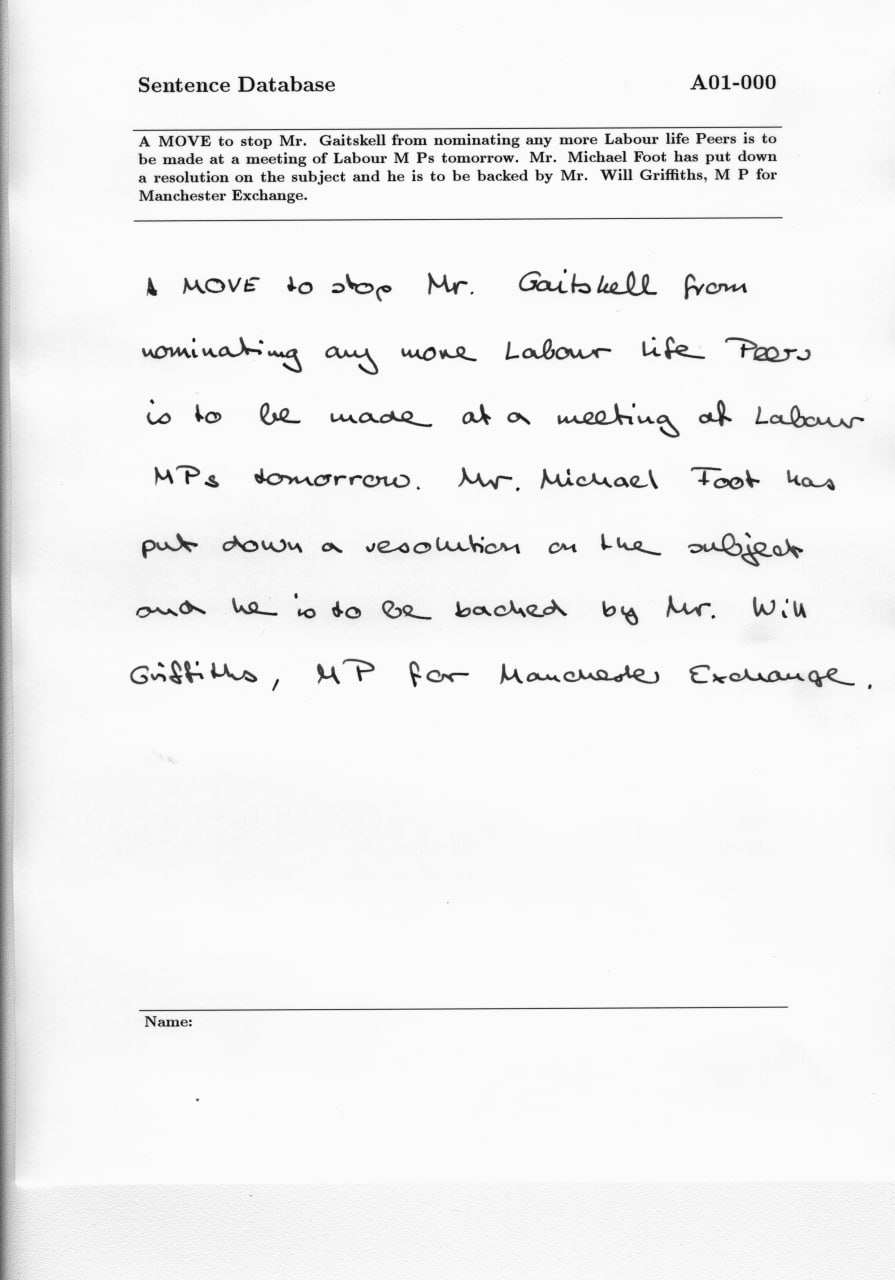
\includegraphics[width=0.45\linewidth]{images/iam_example.jpg}
    \includegraphics[width=0.45\linewidth]{images/hkr_example.png}
    \caption{Примеры изображений из наборов данных IAM (слева) и HKR (справа)}
    \label{fig:dataset_examples}
\end{figure}

Процесс подготовки разных наборов данных для обучения модели отличался незначительно,
так как оба набора данных предоставляют изображения и текстовые аннотации. Наиболее весомым отличием
является структура текстов на изображениях: IAM содержит строки текста, а HKR --- словосочетания.
Данное отличие повлияло на этап предобработки для того, чтобы адаптировать загружаемое изображение
к формату, на котором обучалась модель. Тем не менее, архитектура CRNN позволяет эффективно работать
с обоими типами данных.

\subsection{Подход к анализу эмоций в тексте}

Для анализа эмоций в распознанном тексте был выбран лексиконный подход, который основывается на использовании
заранее размеченного словаря с эмоциональными метками. В качестве такого словаря был выбран словарь эмоций русского языка (RusEmoLex), который
содержит слова и их ассоциации с различными эмоциями. Альтернативой мог бы стать подход на основе машинного обучения, например, с использованием моделей, описанных в \cite{semanticemotion2019}, однако он требует значительно больших размеченных корпусов текстов для обучения.

Преимущество лексиконного подхода заключается в его простоте и прозрачности. Он позволяет быстро определить эмоциональную
окраску текста на основе наличия определенных слов, что подтверждается исследованиями в этой области \cite{anew1999, norms2013}. Однако, этот метод может быть ограничен, так как он не учитывает
контекст и синтаксис, что может привести к ошибкам в определении эмоций, особенно в случае сложных фраз или при наличии отрицаний.

Сложность в применении данного подхода заключается в том, что распознанный текст может содержать ошибки, что затрудняет поиск слов
в лексиконе. Для решения этой проблемы был реализован алгоритм коррекции ошибок распознавания текста на основе триграммного сходства, который позволяет
находить наиболее похожие слова в словаре и использовать их для анализа эмоций. Несмотря на свои ограничения, лексиконный подход
с коррекцией ошибок обеспечивает достаточно хорошую точность для определения доминирующей эмоции в тексте, особенно
при наличии достаточного количества эмоционально окрашенных слов.


\subsection{Вычислительные аспекты обучения сверточной нейронной сети}

Задача по обучению сверточной нейронной сети для распознавания рукописного текста является ресурсоемкой,
так как связана с обработкой матриц и тензоров высокой размерности, особенно при работе с большим количеством
изображений в высоком разрешении. Для решения данных задач традиционно используются графические процессоры, которые
имеют тензорные ядра, оптимизированные для операций линейной алгебры, что позволяет значительно ускорить
обучение по сравнению с выполением аналогичных операций на центральных процессорах.
Обучение модели на современном CPU среднего уровня может занять от нескольких часов до нескольких дней,
в зависимости от объема данных и сложности модели, тогда как на современном GPU это может быть выполнено
за несколько часов.

В рамках проекта обучение проводилось на двух конфигурациях:

\begin{itemize}
    \item AMD Ryzen 5 8400F, 32 ГБ ОЗУ, NVIDIA GeForce GTX 1660 Super 6GB;
    \item AMD Ryzen 5 8400F, 32 ГБ ОЗУ, NVIDIA GeForce RTX 3060 12GB.
\end{itemize}

Обе конфигурации позволили успешно обучить модель, однако видеокарта RTX 3060 позволила увеличить
размер пакета (batch size) и сократить время обучения, что подтверждает важность использования
современного графического процессора (GPU) с большим объемом видеопамяти для задач глубокого обучения.


\begin{table}[H]
\caption{Влияние конфигурации GPU на время обучения}
\label{tab:training_time}
\centering
\small
\renewcommand{\arraystretch}{1.2}
\setlength{\tabcolsep}{6pt}
\begin{tabularx}{0.95\linewidth}{
>{\raggedright\arraybackslash}X
>{\centering\arraybackslash}p{2.0cm}
>{\centering\arraybackslash}p{3.0cm}
>{\centering\arraybackslash}p{3.0cm}
}
\toprule
\textbf{Графический процессор (GPU)} & \textbf{Размер пакета (Batch size)} & \textbf{Высота изображения, px} & \textbf{Время на эпоху} \\
\midrule
NVIDIA GeForce GTX 1660 Super 6GB & 8  & 64  & $\sim$15 минут \\
NVIDIA GeForce RTX 3060 12GB      & 16 & 128 & $\sim$10 минут \\
\bottomrule
\end{tabularx}
\end{table}

Увеличение объема видеопамяти позволило использовать больший размер пакета и обрабатывать
изображения большей высоты, что в итоге сократило время обучения. Это подтверждает,
что для эффективного обучения моделей глубокого обучения в задачах компьютерного зрения
предпочтительно использовать современный графический процессор (GPU).

Также, в ходе экспериментов было замечено, что использование графического процессора (GPU) в SoC Apple M1 Pro
не поддерживается PyTorch для обучения данной модели, что ограничивает возможности ускорения
обучения на данной платформе. Поэтомуболее предпочтительно использовать видеокарты
с поддержкой CUDA для обучения модели, так каксовременные библиотеки глубокого обучения
оптимизированы для работы с такими устройствами.

Обучение модели на центральном процессоре (CPU) не проводилось, так как это было бы крайне неэффективно и заняло бы неприемлемое количество времени.


\section{Выводы}

В ходе выполнения данной работы был разработан программный инструмент, способный
распознавать рукописный текст на русском и английском языках и анализировать
эмоциональную окраску русскоязычного текста. Были решены следующие задачи:
\begin{itemize}
    \item Проанализированы и сравнены существующие подходы к распознаванию рукописного текста, в результате чего была выбрана архитектура сверточно-рекуррентной нейросети (CRNN) как оптимальное решение, обеспечивающее баланс между точностью и вычислительными ресурсами.
    \item Подобраны и подготовлены наборы данных для обучения и тестирования моделей: IAM Handwriting Database для английского языка и HKR Dataset для русского.
    \item Разработана и реализована модель распознавания рукописного текста на основе CRNN с использованием библиотеки PyTorch.
    \item Реализован лексиконный подход к анализу эмоциональной окраски с использованием словаря RusEmoLex и алгоритма коррекции ошибок распознавания текста на основе триграммного сходства.
    \item Создан пользовательский интерфейс, позволяющий удобно работать с программой, выбирать изображения, модели и настраивать параметры обработки.
\end{itemize}

Разработанное программное обеспечение продемонстрировало свою работоспособность на различных системных конфигурациях. Контрольный пример показал, что система успешно справляется с распознаванием текста и анализом эмоций даже при наличии ошибок в исходном распознавании.

Таким образом, цель работы была достигнута. Созданный инструмент может быть использован для автоматической обработки рукописных документов, а также для дальнейших исследований в области анализа тональности текста. Возможными направлениями для дальнейшего развития проекта являются улучшение точности распознавания за счет использования более сложных моделей или расширенных наборов данных, а также добавление поддержки анализа эмоций для других языков.

\clearpage
\addcontentsline{toc}{section}{Список литературы}
\begin{thebibliography}{99}

\bibitem{survey2023}
\href{https://ieeexplore.ieee.org/abstract/document/11303599}
{Handwritten Text Recognition: A Survey.}

\bibitem{ctc2006}
\href{https://www.cs.toronto.edu/~graves/icml_2006.pdf}
{Connectionist Temporal Classification: Labelling Unsegmented Sequence Data with Recurrent Neural Networks.}

\bibitem{mdrnn2008}
\href{https://papers.nips.cc/paper_files/paper/2008/hash/66368270ffd51418ec58bd793f2d9b1b-Abstract.html}
{Offline Handwriting Recognition with Multidimensional Recurrent Neural Networks.}

\bibitem{segmentation2009}
\href{https://users.iit.demokritos.gr/~bgat/Louloud_1_2009.pdf}
{Text line and word segmentation of handwritten documents.}

\bibitem{anew1999}
\href{https://pdodds.w3.uvm.edu/teaching/courses/2009-08UVM-300/docs/others/everything/bradley1999a.pdf}
{Affective Norms for English Words (ANEW).}

\bibitem{norms2013}
\href{https://pubmed.ncbi.nlm.nih.gov/23404613/}
{Norms of valence, arousal, and dominance for 13,915 English lemmas.}

\bibitem{ratings2018}
\href{https://aclanthology.org/P18-1017/}
{Obtaining Reliable Human Ratings of Valence, Arousal, and Dominance for 20,000 English Words.}

\bibitem{scalable2019}
\href{https://ieeexplore.ieee.org/abstract/document/8977983}
{A Scalable Handwritten Text Recognition System.}

\bibitem{database1992}
\href{https://ieeexplore.ieee.org/abstract/document/291440}
{A database for handwritten text recognition research.}

\bibitem{hybridhmm2010}
\href{https://ieeexplore.ieee.org/abstract/document/5551147}
{Improving Offline Handwritten Text Recognition with Hybrid HMM/ANN Models.}

\bibitem{e2eneural2018}
\href{https://arxiv.org/abs/1807.07965}
{An Efficient End-to-End Neural Model for Handwritten Text Recognition.}

\bibitem{semanticemotion2019}
\href{https://ieeexplore.ieee.org/abstract/document/8794541}
{Semantic-Emotion Neural Network for Emotion Recognition From Text.}

\bibitem{rulesemotion2014}
\href{https://ieeexplore.ieee.org/stamp/stamp.jsp?tp=&arnumber=7022622}
{Emotion Recognition from Text Based on Automatically Generated Rules.}

\bibitem{marti2002iam}
\href{https://fki.tic.heia-fr.ch/databases/iam-handwriting-database}
{U. Marti and H. Bunke. The IAM-database:
An English Sentence Database for Off-line
Handwriting Recognition. Int'l Journal on
Document Analysis and Recognition, Volume 5, pages 39--46, 2002.}

\bibitem{hkr2024}
\href{https://link.springer.com/article/10.1007/s11042-021-11399-6}
{Handwritten Kazakh and Russian (HKR) database for text recognition.}
\end{thebibliography}

\end{document}
